
\part{Réplication de données}


\section{État de l'art}
\label{repl:sec:replication}

La maintenance de répliques sur des machines distantes les unes des
autres est un problème ancien. Dès 1975, les bases de données répliquées font
leur apparition~\cite{johnson1975maintenance} afin de résoudre
\begin{inparaenum}[(i)]
\item les problèmes de défaillances~\cite{alsberg1976principle}, i.e., le
  serveur possédant les données étant inaccessible, le client peut contacter
  serveur alternatif connu pour posséder les mêmes données afin de satisfaire sa
  requête;
\item les problèmes de rapidité d'accès, i.e., le client peut contacter un
  serveur dont la latence est la plus faible afin de satisfaire plus rapidement
  sa requête.
\end{inparaenum}

Hélas, avec la réplication, la synchronisation de répliques devient le coeur du
problème. Puisque la communication entre serveurs n'est pas instantanée, les
modifications effectuées sur les données prennent du temps à parvenir aux
répliques. Cela implique des problèmes de
\begin{inparaenum}[(i)]
\item fraîcheur de données -- \emph{est-ce que la donnée que j'obtiens est la
    plus à jour?} -- et de
\item modifications concurrentes -- \emph{avec des modifications effectuées sur
    une même données, au même moment, par deux serveurs distants dont les
    résultats sont différents. Dois-je conserver les deux modifications, ou
    dois-je en privilégier une, ou dois-je employer une autre stratégie?}
\end{inparaenum}


Hélas, d'après le théorème CAP~\cite{gilbert2002brewer} il est impossible de
répliquer sur un grand nombre de serveurs tout en garantissant à la fois :
\begin{itemize}
\item [\textbf{Cohérence :}] un contrat entre le développeur et la structure qui
  spécifie comment cette dernière se comporte suivant les opérations effectuées
  et leur ordonancement.
\item [\textbf{Disponibilité :}] le ratio entre le temps effectif durant lequel
  l'utilisateur accède à un service et le temps durant lequel il souhaite y
  accèder.
\item [\textbf{Tolérance aux pannes :}] les défaillances de serveurs
  n'entrainent pas une panne générale du système.
\end{itemize}

Face à ce constat, deux grandes familles de réplication : la réplication
pessimiste cherche à donner l'illusion d'une donnée unique lorsque la
réplication optimiste autorise à ses répliques de légères divergences
temporaires (cf. §\ref{repl:sec:schemas}). Cette dernière passant plus volontier
à l'échelle, nous nous intéresserons à deux familles d'approches y appartenant,
à savoir les transformés opérationnels dont les opérations sont modifiées à
l'intégration afin d'adapter l'opération au contexte d'exécution, et les
structures de données sans résolution de conflits dont les opérations commutent
(cf. §\ref{repl:sec:otorcrdts}). Finalement, la section~\ref{repl:sec:sequences}
s'intéresse plus particulièrement au type séquence, le plus proche d'un
document.

%%% Local Variables:
%%% mode: latex
%%% TeX-master: "../../paper"
%%% End:

\section{Réplication pessimiste}
\label{repl:sec:pessimistic}

L'objectif de la réplication pessimiste est simple. Il consiste à donner
l'illusion que la donnée manipulée par les utilisateurs est unique,
indépendemment du nombre de répliques réel. Grâce à la réplication pessimiste,
il est facile de raisonner sur les données car leurs spécifications sont proches
de celles proposées dans un \TODO{contexte sans réplications}.

Toutefois, chacune des modifications effectuée doit être validée. L'autorité
décisionnelle diffère en fonction des approches :
\begin{itemize}
\item [\textbf{autorité centrale~\cite{alsberg1976principle} :}] l'un des
  serveurs est désigné responsable d'une donnée. Ceux qui souhaitent modifier la
  donnée sont alors dans l'obligation de demander l'accès exclusif pendant la
  mise en place de cette modification. Dans l'intervalle, les autres répliques
  ne peuvent soumettre de modifications. Enfin, lorsque la modification est
  achevée, la main est rendue au serveur qui peut autoriser d'autres
  modifications. C'est le méchanisme de vérouillage (\emph{lock}).
\item [\textbf{quorum~\cite{gifford1979weighted} :}] les modifications sont
  soumises à un vote où un certains nombre de serveurs \TODO{doivent approuver
    ou non}. \TODO{Serialisation}.
\end{itemize}

La réplication pessimiste est possible lorsque le nombre de répliques est connu,
plutôt petit, et souvent accessible. Ces contraintes sont notamment
satisfaisable dans le \TODO{Nuage}. Les services proposés possèdent d'avantage
d'assurances quant aux résultats de la manipulation des données. Toutefois, de
telles guaranties ne sont pas toujours nécéssaire et leur coût élévée n'est
alors plus justifié. \TODO{La section suivante est.}

%%% Local Variables:
%%% mode: latex
%%% TeX-master: "../../paper"
%%% End:

\section{Réplication optimiste}
\label{repl:sec:optimistic}

En 1987, Demers et al. décrivent une base de données répliquée sur plusieurs
centaines de machines pouvant communiquer entre elles au travers de materiels
aux capacités hétérogènes~\cite{demers1987epidemic}. \TODO{moar.}

La réplication optimiste~\cite{johnson1975maintenance, saito2005optimistic} est
un paradigme de réplication consistant à appliquer les modifications directement
sur la réplique locale.  Ainsi, les données sont toujours disponibles et
réactives aux changements effectués. Ensuite, les modifications sont disséminées
aux autres possesseurs de cette donnée partagée où elles sont appliquées. Au
contraire des approches pessimistes, les approches optimistes ne vérouillent pas
l'accès aux données lors de modifications. En revanche, le critère de cohérence
assuré est plus faible. En particulier, les répliques ont l'autorisation d'avoir
des états temporairement divergeant entre eux :

\begin{itemize}
\item [\textbf{Cohérence à terme :}] lorsque toutes les modifications ont été
  reçues et appliquées par toutes les répliques, celle-ci possèdent un état
  équivalent. Puisque \emph{toutes} les modifications constituent un ensemble
  peu réaliste dans le cadre d'une éxecution réelle, un définition plus précise
  porte sur un sous-ensembles de ces modifications :
\item [\textbf{Cohérence forte à terme~\cite{shapiro2011conflict} :}] les
  répliques ayant réçu et appliqué les même modifications possèdent un état
  équivalent.
\end{itemize}

Ces critères de cohérence posent de nombreux problèmes par leur manque
d'expressivité. En particulier, l'état équivalent vers lequel les répliques
convergent n'est pas spécifié. Celui-ci peut n'avoir aucun lien avec l'éxecution
souhaitée par l'utilisateur. Par exemple, un ensemble dont l'ajout d'éléments
n'a aucun effet converge vers l'ensemble vide. Il maintient donc la cohérence
forte à terme.

\begin{figure}
  \centering
  
\begin{tikzpicture}[scale=1.2]

  \newcommand\X{30pt};
  \newcommand\Y{30pt};
  
  \draw[->](0pt,   0pt)--(10*\X,   0pt);
  \draw[->](0pt, -1*\Y)--(10*\X, -1*\Y);
  \draw[->](0pt, -2*\Y)--(10*\X, -2*\Y);
  
  \draw[fill=black](0pt, 0pt) node[anchor=east]{réplique 1 }circle(2pt);
  \draw[fill=black](0pt, -1*\Y) node[anchor=east]{réplique 2 }circle(2pt);
  \draw[fill=black](0pt, -2*\Y) node[anchor=east]{réplique 3 }circle(2pt);

  \draw(\X,2pt)--node[anchor=south]{[ ]}( \X,   -2pt);
  \draw(\X,2 -1*\Y)--node[anchor=south]{[ ]}(\X,-2 -1*\Y);
  \draw(\X,2 -2*\Y)--node[anchor=south]{[ ]}(\X,-2 -2*\Y);

  \draw(2* \X,2pt)--node[anchor=south]{[QWE]}(2* \X,   -2pt);
%  \draw(2* \X,2 -1*\Y)--node[anchor=south]{[ ]}(2* \X,-2 -1*\Y);
%  \draw(2* \X,2 -2*\Y)--node[anchor=south]{[ ]}(2* \X,-2 -2*\Y);

  \draw[->, dashed] (2*\X, 0pt) -- (8*\X, -1*\Y);
  \draw[->, dashed] (2*\X, 0pt) -- (3*\X, -2*\Y);

  \draw(4*\X, 2 -0*\Y)--node[anchor=south]{[QWE]}(4*\X,-2 -0*\Y);
  \draw(4*\X, 2 -1*\Y)--node[anchor=south]{[ ]}(4*\X,-2 -1*\Y);
  \draw(4*\X, 2 -2*\Y)--node[anchor=south]{[QWE]}(4*\X,-2 -2*\Y);


  \draw(6*\X, 2 -2*\Y)--node[anchor=north]{[QWERTY]}(6*\X,-2 -2*\Y);


  \draw[->, dashed] (6*\X, -2*\Y)--(7*\X, -0*\Y);
  \draw[->, dashed] (6*\X, -2*\Y)--(7*\X, -1*\Y);

  \draw(9*\X, 2 -0*\Y)--node[anchor=south]{[QWERTY]}(9*\X,-2 -0*\Y);
  \draw(9*\X, 2 -1*\Y)--node[anchor=south]{[QWERTY]}(9*\X,-2 -1*\Y);
  \draw(9*\X, 2 -2*\Y)--node[anchor=south]{[QWERTY]}(9*\X,-2 -2*\Y);


%%  \draw[fill=white, very thick]
%%  (0*\X, 0*\Y) node{$p_1$} +(-5pt,-5pt) rectangle +(5pt,5pt);
%%  \draw[->](-5+\X, 5+2*\Y)to[out=120,in=30](0pt,5+2*\Y); %% 6 -> 7
\end{tikzpicture}
  \caption{\label{repl:fig:optimisticexample} Exemple d'éxecution d'un protocole
    de réplication optimiste.}
\end{figure}

La figure~\ref{repl:fig:optimisticexample} présente un cas de séquence
répliquée.  Il existe trois copies d'une séquence initialement vide. La première
copie insère 'QWE' et en dissémine l'information. La troisième copie reçoit
l'opération et l'applique localement. Cette copie insère 'RTY' à la suite de
'QWE' afin d'obtenir 'QWERTY' et envoie l'information aux deux autres
copies. Quel que soit l'ordre de réception, le protocole garanti que les copies
convergent vers un état identique, ici, la séquence 'QWERTY'.

%%% Local Variables:
%%% mode: latex
%%% TeX-master: "../../paper"
%%% End:

\section{Conclusion}

Depuis les premières base de données répliqués, les dimensions ont
considérablement augmentées mais les problématiques restent identiques. Les
réseaux \TODO{pair-à-pair} transforment chaque \TODO{client} en
client-serveur. Chaque utilisateur final possède alors une réplique de la donnée
partagée. Dans ce contexte, il est inenvisageable d'en appeler à la réplication
pessimiste. 

%%% Local Variables:
%%% mode: latex
%%% TeX-master: "../../paper"
%%% End:



\chapter{Structure de données sans résolution de conflits}

\minitoc

\lettrine{L}es structures de données sans résolution de
conflits~\cite{shapiro2011comprehensive} (CRDTs) appartiennent au schéma de
réplication optimiste. \TODO{Ils tirent leur nom de}.  Il en existe deux
familles équivalentes mais proposant un compromis différent :
\begin{itemize}
\item [\textbf{basée sur l'état :}] lors d'une opération, l'état local change et
  est envoyé en totalité aux autres répliques qui fusionnent alors l'état réçu
  et leur état propre. L'envoit d'un état est honéreux et doit être effectué
  avec parcimonie. En revanche, puisqu'il est autonome
  (\TODO{\emph{self-contained}}), il ne requière aucune garantie sur les moyens
  de diffusion.
\item [\textbf{basée sur les opérations :}] lors d'une opération, son résultat
  seul est envoyé aux autres répliques où il est intégré. Les résultats sont
  envoyées les uns après les autres aux cours des opérations ce qui est beaucoup
  moins coûteux que l'état complet. En revanche, cela requière une diffusion
  fiable, i.e., toutes les opérations doivent être inéluctablement reçues par
  toutes les répliques.
\end{itemize}

Dans le reste de ce manuscrit de thèse, nous nous intéresserons plus en détail à
cette seconde famille de structure répliquée. La
section~\ref{crdts:sec:properties} présente les propriétés de ces structures de
données répliquées. La section~\ref{crdts:sec:compteur} décrit les structures
possibles pour le compteur. La section~\ref{crdts:sec:set} décrit les structures
possibles pour les ensembles. Les problèmes de composition de ces structures
sont exposés en section~\ref{crdts:sec:composition}. La
section~\ref{crdts:sec:conclusion} conclue ce chapitre.


%%% Local Variables:
%%% mode: latex
%%% TeX-master: "../../paper"
%%% End:


\section{Propriétés}
\label{crdts:sec:properties}

Selon le formalisme de~\cite{burckhardt2014replicated}, l'implémentation d'un
type de données répliqué $\tau$ est\\
$\mathcal{D}_\tau(\Sigma, \delta_0, M, do, send, receive)$ où \TODO{moar.}

Les structures de données sans résolutions de conflits
fournissent des opérations dont les résultats respectifs commutent à
l'intégration. Ainsi, l'ordre d'intégration des opérations n'importe pas.

%%% Local Variables:
%%% mode: latex
%%% TeX-master: "../../paper"
%%% End:


\section{Compteur}
\section{Ensembles}
\section{Composition}
\section{Conclusion}

\chapter{Séquences répliquées}
\minitoc

%% (TODO) introduction

\section{Transformés opérationnels}
\label{repl:sec:ot}

Les approches à transformés opérationnels~\cite{sun1998operational,
  sun2009contextbased} (OT) sont les plus anciennes et s'appliquent à un large
champs d'applications tels que l'édition de texte, l'édition d'images etc. Dans
le cadre de l'édition de texte, en plus des usuelles opérations d'insertion et
de suppression, OT founit des opérations ciblant les chaînes de caractères
telles que le déplacement, le couper -- coller, etc. Toutefois, l'analyse de
correction nécessite d'examiner chaque paire d'opérations ainsi que leurs
paramètres. En conséquence, lors de l'écriture du papier
\cite{imine2003proving}, peu d'approches étaient réellement correctes. De plus,
cette classe d'approches peut être divisé en deux sous-classes: les approches
centralisées et les approches décentralisées. Les premières réarrangent les
opérations sur un serveur central~\cite{nichols1995high} afin de faciliter la
convergence. Toutefois, la topologie elle-même implique un point individuel de
défaillance, des problèmes de confidentialité, des problèmes d'intelligence
économique, des problèmes de censure, et enfin, de passage à l'échelle. Les
approches décentralisées~\cite{sun2009contextbased}, quant à elle, nécessitent
un vecteur de version afin d'identifier les contextes de génération des
opérations reçues. Elles transforment les arguments de l'opération reçue par
rapport aux opérations concurrentes dans le but d'exécuter de manière cohérente
l'opération sans avoir à défaire et réexecuter ces opérations. De ce fait, bien
que l'exécution locale d'une opération soit très efficace, l'exécution des
opérations reçues est très coûteuse en cas de concurrence. Ainsi, confiné aux
environnements maîtrisés, OT reste efficace~\cite{mehdi2014merging}.

\begin{figure}
  \centering
  
\begin{tikzpicture}[scale=1.2]

  \newcommand\X{30pt};
  \newcommand\Y{30pt};
  
  \draw[->](0pt,   0pt)--(10*\X,   0pt);
  \draw[->](0pt, -1*\Y)--(10*\X, -1*\Y);
  \draw[->](0pt, -2*\Y)--(10*\X, -2*\Y);
  
  \draw[fill=black](0pt, 0pt) node[anchor=east]{réplique 1 }circle(2pt);
  \draw[fill=black](0pt, -1*\Y) node[anchor=east]{réplique 2 }circle(2pt);
  \draw[fill=black](0pt, -2*\Y) node[anchor=east]{réplique 3 }circle(2pt);

  \draw(\X,2pt)--node[anchor=south]{[RTY]}( \X,   -2pt);
  \draw(\X,2 -1*\Y)--node[anchor=south]{[RTY]}(\X,-2 -1*\Y);
  \draw(\X,2 -2*\Y)--node[anchor=south]{[RTY]}(\X,-2 -2*\Y);
  \small
  \draw(3* \X,2pt)--node[anchor=north]{\textsc{insert}(QWE, 0)}(3 * \X,   -2pt);
  \draw(3* \X,2 -2*\Y)--node[anchor=north]{\textsc{delete}(\DARKBLUE{\textbf{0}}, 3)}(3 * \X,-2 -2*\Y);
  \normalsize

  \draw(3* \X,2pt)--node[anchor=south]{[QWERTY]}(3 * \X,   -2pt);
%  \draw(2* \X,2 -1*\Y)--node[anchor=south]{[ ]}(2* \X,-2 -1*\Y)
  \draw(3* \X,2 -2*\Y)--node[anchor=south]{[ ]}( 3 * \X,-2 -2*\Y);

  \draw[->, dashed] (5*\X, 0pt) -- (7*\X, -1*\Y);
  \draw[->, dashed] (5*\X, 0pt) -- (7*\X, -2*\Y);

  \small
  \draw[->, dashed] (5*\X, -2*\Y) -- (7*\X,  0*\Y)
  node[anchor=south]{\textsc{delete}(\DARKBLUE{\textbf{3}}, 3)};
  \normalsize
  \draw[->, dashed] (5*\X, -2*\Y) -- (7*\X, -1*\Y);

  \draw(9*\X, 2 -0*\Y)--node[anchor=south]{[QWE]}(9*\X,-2 -0*\Y);
  \draw(9*\X, 2 -1*\Y)--node[anchor=south]{[QWE]}(9*\X,-2 -1*\Y);
  \draw(9*\X, 2 -2*\Y)--node[anchor=south]{[QWE]}(9*\X,-2 -2*\Y);


%%  \draw(9*\X, 2 -0*\Y)--node[anchor=south]{[QWERTY]}(9*\X,-2 -0*\Y);
%%  \draw(9*\X, 2 -1*\Y)--node[anchor=south]{[QWERTY]}(9*\X,-2 -1*\Y);
%%  \draw(9*\X, 2 -2*\Y)--node[anchor=south]{[QWERTY]}(9*\X,-2 -2*\Y);


%%  \draw[fill=white, very thick]
%%  (0*\X, 0*\Y) node{$p_1$} +(-5pt,-5pt) rectangle +(5pt,5pt);
%%  \draw[->](-5+\X, 5+2*\Y)to[out=120,in=30](0pt,5+2*\Y); %% 6 -> 7
\end{tikzpicture}
  \caption{\label{seq:fig:otexample}Exemple de transformé opérationnel
    garantissant la convergence lors d'opérations concurrentes. L'opération de
    suppression des 3 premiers caractères sur la copie 3 (RTY) est transformée
    afin de supprimer les 3 caractères à l'index 3 sur les autres copies.}
\end{figure}

La figure~\ref{seq:fig:otexample} illustre le principe de fonctionnement des
approches basées sur les transformés opérationnels. Dans ce scenario, les copies
sont toutes initialisées avec la séquence 'RTY'. Ensuite, tandis que la copie 1
insère les 3 caractères 'QWE' en tête de la séquence pour obtenir 'QWERTY', la
copie 3 supprime ses trois caractères pour obtenir la séquence vide. Avant la
dissémination de ces opérations, les copies ne sont pas identiques. Les copies
1, 2, et 3 ont respectivement les séquences [QWERTY], [RTY], []. Lorsque la
copie 1 réçoit l'opération de suppression, elle détecte que cette dernière est
en concurrence avec des opérations déjà intégrées, en l'occurence,
$insert(QWE,\,0)$. Son objectif est alors de déterminer l'impact que cette
opération concurrente a eu sur l'opération réçue afin d'en adapter les
arguments. Ici, l'insertion a décalé la séquence RTY de 3 positions vers la
droite. Par conséquent, La suppression, de part sa position, est elle aussi
décalée de 3 positions vers la droite. La résultat de la transformation est
$delete(3,\,3)$.  La copie 3, lorsqu'elle réçoit l'opération d'insertion,
detecte elle aussi que cette dernière est concurrente. Toutefois, la
transformation est sans effet sur ses arguments. La copie 2, selon l'ordre de
réception, se comporte comme la copie 1 ou la copie 3. À terme, les trois copies
convergent vers une séquence identique 'QWE'.



\section{Pierres tombales}

Les structures de données sans résolution de conflits
(cf. chapitre~\ref{repl:chap:crdts}) pour séquences évitent le coûteux processus
de detection de concurrence. Les approches de cette famille utilisant des
pierres tombales~\cite{ahmed2011evaluating, conway2014language,
  grishchenko2010deep, oster2006data, preguica2009commutative,
  roh2011replicated, weiss2007wooki, wu2010partial, yu2012stringwise} se
caractérisent par la manière dont les suppressions sont traitées. En effet, lors
de l'opération de suppression, ces approches marquent simplement les éléments
supprimés afin de les cacher à l'utilisateur. Bien que supprimées, ces pierres
tombales existent toujours dans la structure représentant la séquence et
continuent d'impacter sur les performances.

\begin{itemize}
\item [\textbf{WOOT~\cite{oster2006data} :}] le premier représentant historique
  des CRDTs pour séquences suivit par deux extensions
  \textbf{WOOTO~\cite{weiss2007wooki}} et
  \textbf{WOOTH~\cite{ahmed2011evaluating}}. Dans cette approche chaque
  identifiant référence les identifiants voisins à l'insertion. Rassemblés, les
  identifiants peuvent être ordonnés grâce à un diagramme de Hasse
  (\REF). Toutefois, cet ordonnancement requière des deux bornes adjacentes
  qu'elles soient déjà intégrées et toujours présentes, d'où les suppressions
  réelles impossibles.

  \begin{figure}
    \centering
    
\begin{tikzpicture}[scale=1.1]

\newcommand\X{ 40pt}
\newcommand\Y{ 30pt}

\draw[fill=white](0 * \X, 0 * \Y) node{$\vdash$}+(-5pt,-5pt)rectangle+(5pt,5pt);
\draw[fill=white](7 * \X, 0 * \Y) node{$\dashv$}+(-5pt,-5pt)rectangle+(5pt,5pt);

\draw[fill=white](1 * \X, 1 * \Y) node{\textbf{Q}}+(-5pt,-5pt)rectangle+(5pt,5pt);
\draw[fill=white](2 * \X, 1 * \Y) node{\textbf{W}}+(-5pt,-5pt)rectangle+(5pt,5pt);

\draw[fill=white](1 * \X, 0 * \Y) node{\textbf{A}}+(-5pt,-5pt)rectangle+(5pt,5pt);
\draw[fill=white, draw=darkblue](2 * \X, 0 * \Y)
node{\DARKBLUE{\textbf{Z}}}+(-5pt,-5pt)rectangle+(5pt,5pt);
\draw[fill=white, draw=blue](3 * \X, 0 * \Y)
node{\BLUE{\textbf{E}}}+(-5pt,-5pt)rectangle+(5pt,5pt);
\draw[fill=white](4 * \X, 0 * \Y) node{\textbf{R}}+(-5pt,-5pt)rectangle+(5pt,5pt);
\draw[fill=white](5 * \X, 0 * \Y) node{\textbf{T}}+(-5pt,-5pt)rectangle+(5pt,5pt);
\draw[fill=white](6 * \X, 0 * \Y) node{\textbf{Y}}+(-5pt,-5pt)rectangle+(5pt,5pt);

\draw[thick](-5+1*\X, -5+0*\Y)--(5+1*\X, 5+0*\Y);
\draw[thick](-5+1*\X, 5+0*\Y)--(5+1*\X, -5+0*\Y);

\draw[thick, color=darkblue](-5+2*\X, -5+0*\Y)--(5+2*\X, 5+0*\Y);
\draw[thick, color=darkblue](-5+2*\X, 5+0*\Y)--(5+2*\X, -5+0*\Y);

\draw[->](1*\X,-5+0*\Y)to[out=-45,in=-135](7*\X, -5+0*\Y);
\draw[->](2*\X,-5+0*\Y)to[out=-45,in=-135](7*\X, -5+0*\Y);
\draw[->](3*\X,-5+0*\Y)to[out=-45,in=-135](7*\X, -5+0*\Y);
\draw[->](4*\X,-5+0*\Y)to[out=-45,in=-135](7*\X, -5+0*\Y);
\draw[->](5*\X,-5+0*\Y)to[out=-45,in=-135](7*\X, -5+0*\Y);
\draw[->](6*\X,-5+0*\Y)to[out=-45,in=-135](7*\X, -5+0*\Y);

\draw[<-](5+0*\X, 0*\Y)--(-5+1*\X, 0*\Y);
\draw[<-, color=darkblue](5+1*\X, 0*\Y)--(-5+2*\X, 0*\Y);
\draw[<-, color=blue](5+2*\X, 0*\Y)--(-5+3*\X, 0*\Y);
\draw[<-](5+3*\X, 0*\Y)--(-5+4*\X, 0*\Y);
\draw[<-](5+4*\X, 0*\Y)--(-5+5*\X, 0*\Y);
\draw[<-](5+5*\X, 0*\Y)--(-5+6*\X, 0*\Y);

\draw[->](1*\X,5+1*\Y)to[out=50,in=130](3*\X, 5+0*\Y);
%\draw[->](2*\X,5+1*\Y)to[out=45,in=135](3*\X, 5+0*\Y);
\draw[->](5+2*\X, 1*\Y)--(3*\X, 5+0*\Y);

\draw[<-](0*\X, 5+0*\Y)--(-5+1*\X, 1*\Y);
\draw[<-](5+1*\X, 1*\Y)--(-5+2*\X, 1*\Y);


\end{tikzpicture}
    \caption{\label{repl:fig:wootexample}Le diagramme de Hasse du modèle WOOT
      représentant la séquence 'QWERTY'. Bien que supprimé, le caractère Z est
      indispensable au bon ordonnancement de la séquence.}
  \end{figure}

  La figure~\ref{repl:fig:wootexample} illustre la nécessité de conserver les
  pierres tombales. Elle montre le diagramme de Hasse généré lors du scenario
  suivant : Tout d'abord, un utilisateur écrit 'AZERTY'. Ensuite, les deux
  premiers caractères sont supprimés afin d'être remplacés par les caractères
  'QW'. La séquence finale est 'QWERTY'. Toutefois, les identifiants ne sont pas
  modifiables, et l'identifiant du caractère 'E' référence l'identifiant de 'Z',
  lui-même référençant l'identifiant de 'A'. Par conséquent, supprimer
  complètement les identifiants de 'A' et/ou de 'Z' revient à rendre
  l'identifiant de 'E' non positionnable, et tout ceux qui en dépendent par
  transitivité.

\item [\textbf{Causal tree~\cite{grishchenko2010deep} :}] caractérise
  explicitement les relations causales grâce à une réprésentation sous forme
  d'arbre. Ainsi, chaque opération est accompagnée de l'identifiant de la
  dernière opération observée. En parcourant l'arbre et en appliquant les
  opérations, la séquence peut être retrouvée. Toutefois, les identifiants sont
  des horloges vectorielles (\emph{vector clock}) dont la taille est prohibitive
  (\REF). De plus, il est nécessaire de conserver tous les noeuds de cet arbre
  causal au cas où une opération y ferait référence.
\item [\textbf{Partial persistent sequence~\cite{wu2010partial} :}] definit les
  identifiants dans l'ensemble des nombres rationnels auxquel est ajoutée une
  limite quant à leur précision. Hélas, cette limite contraint la taille du
  document maximale. \TODO{Moar?}. \TODO{Maybe falls in the other category.}
\item [\textbf{Replicated growable array~\cite{roh2011replicated} :}] représente
  la séquence sous forme de liste supportant les opérations concurrentes. Une
  table de hachage apporte un accès rapide aux éléments grâce à leurs
  identifiants. Les éléments incluent une référence au voisin qu'ils précèdent
  lors de leur insertion. Toutefois, pour ne jamais briser la chaine ainsi
  construite, les éléments supprimés restes présents indéfinitivement mais
  cachés de l'utilisateur. \TODO{Double check.}
\item [\textbf{String-wise~\cite{yu2012stringwise} :}] cible principalement les
  chaines de caractères pouvant être subdivisées lors d'opérations. Les
  identifiants référencent alors les chaines adjacentes à l'insertion ainsi que
  les autres éléments de la chaines si subdivision il y a. De la même manière
  que pour les approches précédentes, les références rendent les suppressions
  réelles impossibles.
\item [\textbf{DiCE~\cite{conway2014language} :}] concentre principalement ses
  efforts sur les garanties de \TODO{\emph{confluence}} de la séquence. Chaque
  identifiant référence le voisin qu'il précède à l'insertion. L'ordre des
  éléments est alors fonction de ces relations de positionnement relatif, et de
  causalité.
\end{itemize}

Bien que l'accent soit mit sur l'impossibilité de réellement supprimer les
éléments de séquences répliquées, toutes ces approches s'avèrent pratiques
lorsque l'historique des opérations doit être conservé. Par exemple, dans le
cadre de l'encyclopédie \emph{Wikipédia}, conserver toutes les modifications
éffectuées permet de recouvrer une version vierge de vandalisme; dans le cadre
du gestionnaire de versions \emph{Git}, il permet de recouvrer une version du
code potentiellement sans erreurs etc. Malheureusement, ces structures
grandissent au moins linéairement comparativement au nombre d'opérations
effectuées sur la séquence. Cela devient paradoxalement problématique, par
exemple, lors de vandalisme où même le contenu indésirable est conservé
indéfinitivement. Survient alors le frustrant constat d'avoir à stocker un
fichier dont le poid ne reflète pas le contenu visible. De plus, les éléments
cachés s'accumulent et dégradent \TODO{continuellement} les performances du
système.

Lorsque conserver l'historique ne constitue pas une contrainte, purger la
structure de données des éléments cachés constitue une solution potentielle aux
dégradations de performances :

\begin{itemize}
\item [\textbf{ramasse-miètes~\cite{abdullahi1998garbage} :}] permet de nettoyer
  une structure de données en vidant de la mémoire les objets qui ne sont plus
  accessibles par le programme. Le contexte \textbf{réparti} étend le cadre du
  programme en considérant le local et le distant. Ainsi, supprimer réellement
  un élément de la séquence revient à s'interroger : \emph{Est-ce que
    \begin{inparaenum}[(i)]
    \item toutes les répliques ont supprimé l'élément et
    \item est-ce que tous les éléments référençant l'élément supprimé ont été
      intégré localement?
    \end{inparaenum}} Cela va sans dire qu'il est difficile d'apporter une
  réponse à ces deux questions. D'autant plus lorsque les possesseurs de
  réplique ne sont pas perpétuellement joignables.
\item [\textbf{core-nebula~\cite{letia2009crdts} :}] propose de contraindre la
  topologie réseau afin de rendre les \TODO{consensus} possibles. Ainsi, un
  coeur décisionnel prend en charge les choix de suppression réelle des objets.
  Ce coeur décisionnel étant restraint à un sous-ensemble des membres du réseaux
  étant toujours accessibles, les décisions peuvent alors être prises de manière
  fiable. Le reste des participants se conforme alors aux décisions prises par
  le coeur \TODO{au risque de perdre certaines de leurs modifications}.
\end{itemize}

La section suivante présente une famille de structures pour séquences dont le
bon fonctionnemement ne requière pas de pierres tombales (\TODO{Treedoc\ldots}).

%%% Local Variables:
%%% mode: latex
%%% TeX-master: "../../paper"
%%% End:


\section{Identifiant de taille variable}

Certaines structures de données sans résolution de conflits pour séquences
utilisent des identifiants dont la taille est variable à la
génération~\cite{andre2013supporting, preguica2009commutative,
  weiss2009logoot}. Ainsi, les identifiants sont toujours uniques et immuables
une fois générés, mais leur structure contient une liste d'éléments encodant
leur position dans la séquence.  Contrairement aux approches basées sur les
pierres tombales, ces identifiants ne dépendent pas d'autres identifiants afin
d'être intégrés. À ce titre, les suppressions peuvent ne se contentent pas de
masquer les éléments, mais les retirent entièrement de la structure. En
revanche, la liste d'éléments constituants les identifiants est susceptible de
grandir \TODO{impactant les performances}. 

\begin{wrapfigure}{r}{0.5\textwidth}
  \vspace{-32pt} %% (ugly)
  \begin{minipage}[t]{0.5\textwidth}
    \begin{algorithm}[H]
      
\footnotesize
\algrenewcommand{\algorithmiccomment}[1]{\hskip2em$\rhd$ #1}

\newcommand{\comment}[1]{$\rhd$ #1}


\algblockdefx[initially]{initially}{endInitially}
[0] {\textbf{INITIALLY:}} 

\algblockdefx[local]{local}{endLocal}
[0] {\textbf{LOCAL UPDATE:}}

\algsetblockdefx[received]{received}{endReceived}
{65535}{}
[0] {\textbf{RECEIVED UPDATE:}}

\algblockdefx[onInsert]{onLocal}{endOnLocal}
[0] {\textbf{on} insert ($\DARKBLUE{p \in \mathcal{I}},\,\alpha \in \mathcal{A},\,
  \DARKBLUE{q\in\mathcal{I}}$):}
[0] {\textbf{on} delete ($i \in \mathcal{I}$):} 

\algblockdefx[onRemote]{onRemote}{endOnRemote}
[0] {\textbf{on} insert ($i\in\mathcal{I}$):\hfill\comment{once per identifier}}
[0] {\textbf{on} delete ($i\in\mathcal{I}$):\hfill\comment{$i$ has been integrated}}

\newcommand{\LINEFOR}[2]{%
  \algorithmicfor\ {#1}\ \algorithmicdo\ {#2} %
}

\newcommand{\LINEIFTHEN}[2]{%
  \algorithmicif\ {#1}\ \algorithmicthen\ {#2} %
}

\newcommand{\INDSTATE}[1][1]{\State\hspace{\algorithmicindent}}

\begin{algorithmic}[1]
  \Statex
  \initially
    \State $\mathcal{T} \leftarrow \varnothing$; \hfill \comment{the CRDT}
  \endInitially
  
  \local
    \onLocal
    \State \textbf{let} $path \leftarrow \DARKBLUE{\textsc{allocPath}(p.P,\,q.P)}$; \label{line:allocpath}
    \State \textbf{let} $dis \leftarrow \textsc{allocDis}(p,\, path,\, q)$; \label{line:allocdes}
    \State $\textsc{broadcast}('insert',\, \langle path,\, \alpha,\, dis \rangle)$;
    \endOnLocal
    \INDSTATE $\textsc{broadcast}('delete',\,i)$;
  \endLocal
  
  \received
    \onRemote
    \State $\mathcal{T} \leftarrow \mathcal{T} \cup i$;
    \endOnRemote
    \INDSTATE $\mathcal{T} \leftarrow \mathcal{T}\, \backslash\, i$; 
  
\end{algorithmic}

      \caption{\label{repl:algo:crdtabstract} Squelette.}
    \end{algorithm}
  \end{minipage}
  \vspace{-32pt}
\end{wrapfigure}

\TODO{Definir le modèle.}

L'algorithme~\ref{repl:algo:crdtabstract} présente le squelette de cette famille
de structure pour séquence.  Il est divisé en deux parties qui correspondent à
l'exécution locale et l'exécution distante de la réplication
optimiste. Celles-ci sont elles-mêmes divisées en deux types d'évènements
correspondant aux opérations d'insertions et de suppression d'un
élément. L'algorithme met en lumière trois points :

\begin{itemize}
\item [\textbf{signature :}] les opérations sur la séquence répliquée prennent
  pour arguments les identifiants adjacents à l'insertion, au lieu d'un indice
  dans la séquence pour les séquences \TODO{classiques}.
\end{itemize}

\begin{itemize}
\item [\textbf{complexité locale :}] la complexité de l'algorithme est répartie
  entre la génération d'un identifiant locale et son intégration à la structure
  en partie distante.
\item [\textbf{allocation de chemin} :] la taille des identifiants dépend
  principalement de l'allocation d'un chemin dans l'arbre
  (cf. ligne~\ref{line:allocpath}) auquel est ajouté un désambiguateur
  (cf. ligne~\ref{line:allocdes}) afin de garantir l'unicité de l'identifiant.
\end{itemize}

% \begin{figure*}
%   \centering
%   \subfloat[Allocation quasi-optimale]
%   [\label{fig:lseq:allocpathexampleA}Cas d'une allocation quasi-optimale]
%   {\begin{tikzpicture}[scale=1.2]

  %% node to node
  \small
  \draw[dashed, thick] (0pt,0pt) -- node[anchor=south east]{0} (-70pt,-40pt);
  \draw[thick] (0pt,0pt) -- node[anchor=east]{\DARKBLUE{1}} (-50pt,-40pt);
  \draw[thick] (0pt,0pt) -- node[anchor=east]{\DARKBLUE{2}} (-30pt,-40pt);
  \draw[thick] (0pt,0pt) -- node[anchor=east]{\DARKBLUE{3}} (-10pt,-40pt);
  \draw[thick] (0pt,0pt) -- node[anchor=west]{\DARKBLUE{4}} ( 10pt,-40pt);
  \draw[thick] (0pt,0pt) -- node[anchor=west]{\DARKBLUE{5}} ( 30pt,-40pt);
  \draw[thick] (0pt,0pt) -- node[anchor=west]{\DARKBLUE{6}} ( 50pt,-40pt);
  \draw[dashed, thick] (0pt,0pt) -- node[anchor=south west]{9} ( 70pt,-40pt);

  %% node to element
  \draw[->] (-50pt,-40pt) -- (-50pt,-50pt);
  \draw[->] (-30pt,-40pt) -- (-30pt,-50pt);
  \draw[->] (-10pt,-40pt) -- (-10pt,-50pt);
  \draw[->] ( 10pt,-40pt) -- ( 10pt,-50pt);
  \draw[->] ( 30pt,-40pt) -- ( 30pt,-50pt);
  \draw[->] ( 50pt,-40pt) -- ( 50pt,-50pt);

  %% element to desambiguator
  \draw[->,densely dashdotted] ( -50pt,-58pt) -- ( -50pt,-68.5pt);
  \draw[->,densely dashdotted] ( -30pt,-58pt) -- ( -30pt,-68.5pt);
  \draw[->,densely dashdotted] ( -10pt,-58pt) -- ( -10pt,-68.5pt);
  \draw[->,densely dashdotted] (  10pt,-58pt) -- (  10pt,-68.5pt);
  \draw[->,densely dashdotted] (  30pt,-58pt) -- (  30pt,-68.5pt);
  \draw[->,densely dashdotted] (  50pt,-58pt) -- (  50pt,-68.5pt);

  \draw[fill=black] (  0pt,  0pt) circle (1pt);
  \draw[fill=black] (-70pt,-40pt) circle (1pt);
  \draw[fill=white] (-50pt,-40pt) circle (1pt);
  \draw[fill=white] (-30pt,-40pt) circle (1pt);
  \draw[fill=white] (-10pt,-40pt) circle (1pt);
  \draw[fill=white] ( 10pt,-40pt) circle (1pt);
  \draw[fill=white] ( 30pt,-40pt) circle (1pt);
  \draw[fill=white] ( 50pt,-40pt) circle (1pt);
  \draw[fill=black] ( 70pt,-40pt) circle (1pt);

  %% elements
  \draw[fill=white](-50pt,-54pt)
  node{\textbf{Q}}+(-4pt,-4pt)rectangle+(4pt,4pt) ;
  \draw[fill=white](50pt,-54pt)
  node{\textbf{Y}} +(-4pt,-4pt) rectangle +(4pt,4pt) ;
  \draw[fill=white]( 10pt,-54pt)
  node{\textbf{R}} +(-4pt,-4pt) rectangle +(4pt,4pt) ;
  \draw[fill=white] ( -30pt,-54pt)
  node{\textbf{W}} +(-4pt,-4pt) rectangle +(4pt,4pt) ;
  \draw[fill=white] ( -10pt,-54pt)
  node{\textbf{E}} +(-4pt,-4pt) rectangle +(4pt,4pt) ;
  \draw[fill=white]( 30pt,-54pt)
  node{\textbf{T}} +(-4pt,-4pt) rectangle +(4pt,4pt) ;

  %% desambiguator
  \draw[fill=gray!20] (-50pt,-71pt) +(-2.5pt,-2.5pt) rectangle +(2.5pt,2.5pt);
  \draw[fill=gray!20] (-30pt,-71pt) +(-2.5pt,-2.5pt) rectangle +(2.5pt,2.5pt);
  \draw[fill=gray!20] (-10pt,-71pt) +(-2.5pt,-2.5pt) rectangle +(2.5pt,2.5pt);
  \draw[fill=gray!20] ( 10pt,-71pt) +(-2.5pt,-2.5pt) rectangle +(2.5pt,2.5pt);
  \draw[fill=gray!20] ( 30pt,-71pt) +(-2.5pt,-2.5pt) rectangle +(2.5pt,2.5pt);
  \draw[fill=gray!20] ( 50pt,-71pt) +(-2.5pt,-2.5pt) rectangle +(2.5pt,2.5pt);

  %% insertion order
  \draw[->,dashed] (-50pt, -90pt) -- node[anchor=north]{insertion order}
  (50pt, -90pt);

\end{tikzpicture}
}
%   \hspace{40pt}
%   \subfloat[Pire cas d'allocation]
%   [Pire cas d'allocation]
%   {\begin{tikzpicture}[scale=1.2]

\newcommand\Y{-19}
\newcommand\ADDY{-8}

  %% node to node
  \small
  \draw[thick] (0pt,0pt) -- node[anchor=south east]{\DARKBLUE{0}} (-40pt,\Y pt);
  \draw[thick] (0pt,0pt) -- node[anchor=east]{1} (30pt, \Y pt); %% Y
  \draw[thick] (-40pt, \Y pt) -- node[anchor=north]{1} (15pt, 2 * \Y pt); %% T
  \draw[thick] (-40pt, \Y pt) -- node[anchor=east]{\DARKBLUE{0}} (-40pt, 2 * \Y pt); %% 0
  \draw[thick] (-40pt, 2*\Y pt) -- node[anchor=north]{1} (0pt, 3 * \Y pt); %% R
  \draw[thick] (-40pt, 2*\Y pt)-- node[anchor=east]{\DARKBLUE{0}}(-40pt, 3 * \Y pt); %% 0
  \draw[thick] (-40pt, 3*\Y pt) -- node[anchor=north]{1}(-15pt,4 * \Y pt); %% E
  \draw[thick] (-40pt, 3*\Y pt) -- node[anchor=east]{\DARKBLUE{0}}(-40pt,4 * \Y pt); %% 0
  \draw[thick] (-40pt, 4*\Y pt) -- node[anchor=north]{1}(-25pt,5 * \Y pt); %% W
  \draw[thick] (-40pt, 4*\Y pt) -- node[anchor=east]{\DARKBLUE{0}}(-40pt,5 * \Y pt); %% 0
  \draw[thick] (-40pt, 5*\Y pt) -- node[anchor=east]{\DARKBLUE{1}}(-35pt,6 * \Y pt); %% Q

  \draw[dashed, thick] (0pt,0pt) -- node[anchor=south west]{9} (40pt,\Y pt);

  %% node to element
  \draw[->] ( 30pt, \Y pt) -- ( 30pt, \ADDY + \Y pt); %% Y
  \draw[->] ( 15pt, 2* \Y pt) -- ( 15pt, \ADDY + 2 *\Y pt); %% T
  \draw[->] (  0pt, 3 *\Y pt) -- (  0pt, \ADDY + 3 *\Y pt); %% R
  \draw[->] (-15pt, 4 *\Y pt) -- ( -15pt, \ADDY + 4 *\Y pt); %% E
  \draw[->] (-25pt, 5 *\Y pt) -- ( -25pt, \ADDY + 5 *\Y pt); %% W
  \draw[->] (-35pt, 6 *\Y pt) -- ( -35pt, \ADDY + 6 *\Y pt); %% Q

  %% element to desambiguator
  \draw[->,densely dashdotted]
  ( 30pt, \ADDY + \Y pt) -- ( 30pt,2.75*\ADDY+\Y pt); %% Y
  \draw[->,densely dashdotted]
  ( 15pt, \ADDY + 2* \Y pt) -- ( 15pt,2.75*\ADDY+ 2* \Y pt); %% T
  \draw[->,densely dashdotted]
  ( 0pt, \ADDY + 3* \Y pt) -- (  0pt,2.75*\ADDY+ 3* \Y pt); %% R
  \draw[->,densely dashdotted]
  ( -15pt, \ADDY + 4 *\Y pt) -- ( -15pt,2.75*\ADDY+ 4* \Y pt); %% E
  \draw[->,densely dashdotted]
  ( -25pt, \ADDY + 5 *\Y pt) -- ( -25pt,2.75*\ADDY+ 5*\Y pt); %% W
  \draw[->,densely dashdotted]
  ( -35pt, \ADDY + 6* \Y pt) -- ( -35pt,2.75*\ADDY+ 6*\Y pt); %% Q

  %% node
  \draw[fill=black] (0pt,0pt) circle (1pt); %% rooot
  \draw[fill=white] ( 30pt, \Y pt) circle (1pt); %% Y
  \draw[fill=white] (-40pt, \Y pt) circle (1pt); %% 0
  \draw[fill=white] ( 15 pt, 2 * \Y pt) circle (1pt); %% T
  \draw[fill=white] (-40pt, 2 * \Y pt) circle (1pt); %% 0
  \draw[fill=white] (  0 pt, 3 * \Y pt) circle (1pt); %% R
  \draw[fill=white] (-40pt, 3 * \Y pt) circle (1pt); %% 0
  \draw[fill=white] (-15 pt, 4 * \Y pt) circle (1pt); %% E
  \draw[fill=white] (-40pt, 4 * \Y pt) circle (1pt); %% 0
  \draw[fill=white] (-25 pt, 5 * \Y pt) circle (1pt); %% W
  \draw[fill=white] (-40pt, 5 * \Y pt) circle (1pt); %% 0
  \draw[fill=white] (-35 pt, 6 * \Y pt) circle (1pt); %% Q

  \draw[fill=black] ( 40pt, \Y pt) circle (1pt);


  %% elements
  \draw[fill=white] ( 30pt, -4 + \ADDY + \Y pt)
  node{\textbf{Y}} +(-4pt,-4pt) rectangle +(4pt,4pt) ; %% Y
  \draw[fill=white] ( 15pt, -4 + \ADDY +  2 *\Y pt)
  node{\textbf{T}} +(-4pt,-4pt) rectangle +(4pt,4pt) ; %% T
  \draw[fill=white] (  0pt, -4 + \ADDY +  3* \Y pt)
  node{\textbf{R}} +(-4pt,-4pt) rectangle +(4pt,4pt) ; %% R
  \draw[fill=white] (-15pt, -4 + \ADDY + 4 *\Y pt)
  node{\textbf{E}} +(-4pt,-4pt) rectangle +(4pt,4pt) ; %% E
  \draw[fill=white] (-25pt, -4 + \ADDY + 5 * \Y pt)
  node{\textbf{W}} +(-4pt,-4pt) rectangle +(4pt,4pt) ; %% W
  \draw[fill=white] (-35pt, -4 + \ADDY + 6 *\Y pt)
  node{\textbf{Q}} +(-4pt,-4pt) rectangle +(4pt,4pt) ; %% Q

  %% desambiguator
  \draw[fill=gray!20]( 30pt, -2.5 + 2.75 * \ADDY + \Y pt)
  +(-2.5pt,-2.5pt) rectangle +(2.5pt,2.5pt);
  \draw[fill=gray!20]( 15pt, -2.5 + 2.75 * \ADDY +2 *\Y pt)
  +(-2.5pt,-2.5pt) rectangle +(2.5pt,2.5pt);
  \draw[fill=gray!20](  0pt, -2.5 + 2.75 * \ADDY + 3*\Y pt)
  +(-2.5pt,-2.5pt) rectangle +(2.5pt,2.5pt);
  \draw[fill=gray!20](-15pt, -2.5 + 2.75 * \ADDY +4*\Y pt )
  +(-2.5pt,-2.5pt) rectangle +(2.5pt,2.5pt);
  \draw[fill=gray!20](-25pt, -2.5 + 2.75 * \ADDY + 5*\Y pt)
  +(-2.5pt,-2.5pt) rectangle +(2.5pt,2.5pt);
  \draw[fill=gray!20](-35pt, -2.5 + 2.75 * \ADDY +6*\Y pt) 
  +(-2.5pt,-2.5pt) rectangle +(2.5pt,2.5pt);

  %% insertion order
  \draw[->,dashed] (30pt, 3 * \Y pt) -- node[anchor=west,align=left]
  {\ \ insertion\\ order} (-25pt, 7.5 * \Y pt);

\end{tikzpicture}
}
%   \caption{\label{fig:lseq:allocpathexample} Deux arbres remplis d'identifiants
%     résultant de deux séquences d'édition différentes et dont la séquence finale
%     est identique : $QWERTY$. L'allocation des identifiants se fait selon le
%     même algorithme qui alloue la branche la plus à gauche de l'arbre. L'arbre
%     quasiment optimal ne possède que des branches de profondeur 1 tandis que
%     l'arbre pire cas atteint une profondeur de 6.}
% \end{figure*}

Les figures~\ref{repl:fig:allocpathexampleA} et~\ref{repl:fig:allocpathexampleB}
illustrent les difficultés rencontrées lors de l'allocation des chemins
composant les identifiants. Les structures d'arbre permettant de représenter les
séquences utilisent les fonctions d'allocation suivantes : la branche la plus à
gauche, et la plus petite profondeur de l'arbre possible. Dans les deux cas, la
séquence finale est 'QWERTY'. Toutefois, les lettres ne sont pas insérées dans
un ordre identique. Dans le premier cas, 'Q' est inséré à l'index 0, suivit de
'W' à l'index 1, suivit de 'E' à l'index 2 etc. Cette séquence d'opérations
d'insertions $[(Q,\,0)$, $(W,\,1)$, $(E,\,2)$\ldots$]$ est nommée \emph{séquence
  d'édition}. Dans le second cas, la lettre 'Y' est insérée à l'index 0, suivit
du 'T' à l'index 0 qui va décaler le 'Y' en index 1, etc. La séquence d'édition
qui correspond à ce cas est : $[(Y,\,0)$, $(T,\,0)$, $(R,\,0)$\ldots$]$.

\begin{wrapfigure}{r}{0.5\textwidth}
  \vspace{-15pt}
  \centering
  \begin{tikzpicture}[scale=1.2]

  %% node to node
  \small
  \draw[dashed, thick] (0pt,0pt) -- node[anchor=south east]{0} (-70pt,-40pt);
  \draw[thick] (0pt,0pt) -- node[anchor=east]{\DARKBLUE{1}} (-50pt,-40pt);
  \draw[thick] (0pt,0pt) -- node[anchor=east]{\DARKBLUE{2}} (-30pt,-40pt);
  \draw[thick] (0pt,0pt) -- node[anchor=east]{\DARKBLUE{3}} (-10pt,-40pt);
  \draw[thick] (0pt,0pt) -- node[anchor=west]{\DARKBLUE{4}} ( 10pt,-40pt);
  \draw[thick] (0pt,0pt) -- node[anchor=west]{\DARKBLUE{5}} ( 30pt,-40pt);
  \draw[thick] (0pt,0pt) -- node[anchor=west]{\DARKBLUE{6}} ( 50pt,-40pt);
  \draw[dashed, thick] (0pt,0pt) -- node[anchor=south west]{9} ( 70pt,-40pt);

  %% node to element
  \draw[->] (-50pt,-40pt) -- (-50pt,-50pt);
  \draw[->] (-30pt,-40pt) -- (-30pt,-50pt);
  \draw[->] (-10pt,-40pt) -- (-10pt,-50pt);
  \draw[->] ( 10pt,-40pt) -- ( 10pt,-50pt);
  \draw[->] ( 30pt,-40pt) -- ( 30pt,-50pt);
  \draw[->] ( 50pt,-40pt) -- ( 50pt,-50pt);

  %% element to desambiguator
  \draw[->,densely dashdotted] ( -50pt,-58pt) -- ( -50pt,-68.5pt);
  \draw[->,densely dashdotted] ( -30pt,-58pt) -- ( -30pt,-68.5pt);
  \draw[->,densely dashdotted] ( -10pt,-58pt) -- ( -10pt,-68.5pt);
  \draw[->,densely dashdotted] (  10pt,-58pt) -- (  10pt,-68.5pt);
  \draw[->,densely dashdotted] (  30pt,-58pt) -- (  30pt,-68.5pt);
  \draw[->,densely dashdotted] (  50pt,-58pt) -- (  50pt,-68.5pt);

  \draw[fill=black] (  0pt,  0pt) circle (1pt);
  \draw[fill=black] (-70pt,-40pt) circle (1pt);
  \draw[fill=white] (-50pt,-40pt) circle (1pt);
  \draw[fill=white] (-30pt,-40pt) circle (1pt);
  \draw[fill=white] (-10pt,-40pt) circle (1pt);
  \draw[fill=white] ( 10pt,-40pt) circle (1pt);
  \draw[fill=white] ( 30pt,-40pt) circle (1pt);
  \draw[fill=white] ( 50pt,-40pt) circle (1pt);
  \draw[fill=black] ( 70pt,-40pt) circle (1pt);

  %% elements
  \draw[fill=white](-50pt,-54pt)
  node{\textbf{Q}}+(-4pt,-4pt)rectangle+(4pt,4pt) ;
  \draw[fill=white](50pt,-54pt)
  node{\textbf{Y}} +(-4pt,-4pt) rectangle +(4pt,4pt) ;
  \draw[fill=white]( 10pt,-54pt)
  node{\textbf{R}} +(-4pt,-4pt) rectangle +(4pt,4pt) ;
  \draw[fill=white] ( -30pt,-54pt)
  node{\textbf{W}} +(-4pt,-4pt) rectangle +(4pt,4pt) ;
  \draw[fill=white] ( -10pt,-54pt)
  node{\textbf{E}} +(-4pt,-4pt) rectangle +(4pt,4pt) ;
  \draw[fill=white]( 30pt,-54pt)
  node{\textbf{T}} +(-4pt,-4pt) rectangle +(4pt,4pt) ;

  %% desambiguator
  \draw[fill=gray!20] (-50pt,-71pt) +(-2.5pt,-2.5pt) rectangle +(2.5pt,2.5pt);
  \draw[fill=gray!20] (-30pt,-71pt) +(-2.5pt,-2.5pt) rectangle +(2.5pt,2.5pt);
  \draw[fill=gray!20] (-10pt,-71pt) +(-2.5pt,-2.5pt) rectangle +(2.5pt,2.5pt);
  \draw[fill=gray!20] ( 10pt,-71pt) +(-2.5pt,-2.5pt) rectangle +(2.5pt,2.5pt);
  \draw[fill=gray!20] ( 30pt,-71pt) +(-2.5pt,-2.5pt) rectangle +(2.5pt,2.5pt);
  \draw[fill=gray!20] ( 50pt,-71pt) +(-2.5pt,-2.5pt) rectangle +(2.5pt,2.5pt);

  %% insertion order
  \draw[->,dashed] (-50pt, -90pt) -- node[anchor=north]{insertion order}
  (50pt, -90pt);

\end{tikzpicture}

  \caption{\label{repl:fig:allocpathexampleA}Allocation quasi-optimale}
  \vspace{-15pt}
\end{wrapfigure}

\textbf{Premier cas :} la fonction $allocPath$ alloue la branche la plus à
gauche possible. Par conséquent, la séquence d'édition $[(Q,\,0)$, $(W,\,1)$,
$(E,\,2)$\ldots$]$ conduit aux chemins suivant $\langle [1],\,Q\rangle$,
$\langle [2],\, W \rangle$, $\langle [3],\, E\rangle$, etc. Dans ce cas, la
profondeur de l'arbre n'augmente jamais. À cet égard, la fonction $allocPath$
est très efficace. Cependant, elle n'est pas totalement optimale puisque pour
l'arbre est prévu pour accueillir 8 identifiants lorsque seulement 6 sont
alloués.

\begin{wrapfigure}{r}{0.5\textwidth}
  \vspace{-15pt}
  \centering
  \begin{tikzpicture}[scale=1.2]

\newcommand\Y{-19}
\newcommand\ADDY{-8}

  %% node to node
  \small
  \draw[thick] (0pt,0pt) -- node[anchor=south east]{\DARKBLUE{0}} (-40pt,\Y pt);
  \draw[thick] (0pt,0pt) -- node[anchor=east]{1} (30pt, \Y pt); %% Y
  \draw[thick] (-40pt, \Y pt) -- node[anchor=north]{1} (15pt, 2 * \Y pt); %% T
  \draw[thick] (-40pt, \Y pt) -- node[anchor=east]{\DARKBLUE{0}} (-40pt, 2 * \Y pt); %% 0
  \draw[thick] (-40pt, 2*\Y pt) -- node[anchor=north]{1} (0pt, 3 * \Y pt); %% R
  \draw[thick] (-40pt, 2*\Y pt)-- node[anchor=east]{\DARKBLUE{0}}(-40pt, 3 * \Y pt); %% 0
  \draw[thick] (-40pt, 3*\Y pt) -- node[anchor=north]{1}(-15pt,4 * \Y pt); %% E
  \draw[thick] (-40pt, 3*\Y pt) -- node[anchor=east]{\DARKBLUE{0}}(-40pt,4 * \Y pt); %% 0
  \draw[thick] (-40pt, 4*\Y pt) -- node[anchor=north]{1}(-25pt,5 * \Y pt); %% W
  \draw[thick] (-40pt, 4*\Y pt) -- node[anchor=east]{\DARKBLUE{0}}(-40pt,5 * \Y pt); %% 0
  \draw[thick] (-40pt, 5*\Y pt) -- node[anchor=east]{\DARKBLUE{1}}(-35pt,6 * \Y pt); %% Q

  \draw[dashed, thick] (0pt,0pt) -- node[anchor=south west]{9} (40pt,\Y pt);

  %% node to element
  \draw[->] ( 30pt, \Y pt) -- ( 30pt, \ADDY + \Y pt); %% Y
  \draw[->] ( 15pt, 2* \Y pt) -- ( 15pt, \ADDY + 2 *\Y pt); %% T
  \draw[->] (  0pt, 3 *\Y pt) -- (  0pt, \ADDY + 3 *\Y pt); %% R
  \draw[->] (-15pt, 4 *\Y pt) -- ( -15pt, \ADDY + 4 *\Y pt); %% E
  \draw[->] (-25pt, 5 *\Y pt) -- ( -25pt, \ADDY + 5 *\Y pt); %% W
  \draw[->] (-35pt, 6 *\Y pt) -- ( -35pt, \ADDY + 6 *\Y pt); %% Q

  %% element to desambiguator
  \draw[->,densely dashdotted]
  ( 30pt, \ADDY + \Y pt) -- ( 30pt,2.75*\ADDY+\Y pt); %% Y
  \draw[->,densely dashdotted]
  ( 15pt, \ADDY + 2* \Y pt) -- ( 15pt,2.75*\ADDY+ 2* \Y pt); %% T
  \draw[->,densely dashdotted]
  ( 0pt, \ADDY + 3* \Y pt) -- (  0pt,2.75*\ADDY+ 3* \Y pt); %% R
  \draw[->,densely dashdotted]
  ( -15pt, \ADDY + 4 *\Y pt) -- ( -15pt,2.75*\ADDY+ 4* \Y pt); %% E
  \draw[->,densely dashdotted]
  ( -25pt, \ADDY + 5 *\Y pt) -- ( -25pt,2.75*\ADDY+ 5*\Y pt); %% W
  \draw[->,densely dashdotted]
  ( -35pt, \ADDY + 6* \Y pt) -- ( -35pt,2.75*\ADDY+ 6*\Y pt); %% Q

  %% node
  \draw[fill=black] (0pt,0pt) circle (1pt); %% rooot
  \draw[fill=white] ( 30pt, \Y pt) circle (1pt); %% Y
  \draw[fill=white] (-40pt, \Y pt) circle (1pt); %% 0
  \draw[fill=white] ( 15 pt, 2 * \Y pt) circle (1pt); %% T
  \draw[fill=white] (-40pt, 2 * \Y pt) circle (1pt); %% 0
  \draw[fill=white] (  0 pt, 3 * \Y pt) circle (1pt); %% R
  \draw[fill=white] (-40pt, 3 * \Y pt) circle (1pt); %% 0
  \draw[fill=white] (-15 pt, 4 * \Y pt) circle (1pt); %% E
  \draw[fill=white] (-40pt, 4 * \Y pt) circle (1pt); %% 0
  \draw[fill=white] (-25 pt, 5 * \Y pt) circle (1pt); %% W
  \draw[fill=white] (-40pt, 5 * \Y pt) circle (1pt); %% 0
  \draw[fill=white] (-35 pt, 6 * \Y pt) circle (1pt); %% Q

  \draw[fill=black] ( 40pt, \Y pt) circle (1pt);


  %% elements
  \draw[fill=white] ( 30pt, -4 + \ADDY + \Y pt)
  node{\textbf{Y}} +(-4pt,-4pt) rectangle +(4pt,4pt) ; %% Y
  \draw[fill=white] ( 15pt, -4 + \ADDY +  2 *\Y pt)
  node{\textbf{T}} +(-4pt,-4pt) rectangle +(4pt,4pt) ; %% T
  \draw[fill=white] (  0pt, -4 + \ADDY +  3* \Y pt)
  node{\textbf{R}} +(-4pt,-4pt) rectangle +(4pt,4pt) ; %% R
  \draw[fill=white] (-15pt, -4 + \ADDY + 4 *\Y pt)
  node{\textbf{E}} +(-4pt,-4pt) rectangle +(4pt,4pt) ; %% E
  \draw[fill=white] (-25pt, -4 + \ADDY + 5 * \Y pt)
  node{\textbf{W}} +(-4pt,-4pt) rectangle +(4pt,4pt) ; %% W
  \draw[fill=white] (-35pt, -4 + \ADDY + 6 *\Y pt)
  node{\textbf{Q}} +(-4pt,-4pt) rectangle +(4pt,4pt) ; %% Q

  %% desambiguator
  \draw[fill=gray!20]( 30pt, -2.5 + 2.75 * \ADDY + \Y pt)
  +(-2.5pt,-2.5pt) rectangle +(2.5pt,2.5pt);
  \draw[fill=gray!20]( 15pt, -2.5 + 2.75 * \ADDY +2 *\Y pt)
  +(-2.5pt,-2.5pt) rectangle +(2.5pt,2.5pt);
  \draw[fill=gray!20](  0pt, -2.5 + 2.75 * \ADDY + 3*\Y pt)
  +(-2.5pt,-2.5pt) rectangle +(2.5pt,2.5pt);
  \draw[fill=gray!20](-15pt, -2.5 + 2.75 * \ADDY +4*\Y pt )
  +(-2.5pt,-2.5pt) rectangle +(2.5pt,2.5pt);
  \draw[fill=gray!20](-25pt, -2.5 + 2.75 * \ADDY + 5*\Y pt)
  +(-2.5pt,-2.5pt) rectangle +(2.5pt,2.5pt);
  \draw[fill=gray!20](-35pt, -2.5 + 2.75 * \ADDY +6*\Y pt) 
  +(-2.5pt,-2.5pt) rectangle +(2.5pt,2.5pt);

  %% insertion order
  \draw[->,dashed] (30pt, 3 * \Y pt) -- node[anchor=west,align=left]
  {\ \ insertion\\ order} (-25pt, 7.5 * \Y pt);

\end{tikzpicture}

  \caption{\label{repl:fig:allocpathexampleB}Allocation pire-cas}
  \vspace{-20pt}
\end{wrapfigure}


\textbf{Second cas :} la séquence d'édition $[(Y,\,0)$, $(T,\,0)$,
$(R,\,0)$\ldots$]$ implique une augmentation de la profondeur de l'arbre à
chaque nouvelle insertion d'élément. En effet, le chemin est choisit est
toujours celui qui est le petit possible. Les éléments suivant ne bénéficie pas
de suffisamment de place à la profondeur courante de l'arbre, d'où la nécessité
d'augmenter sa profondeur. Les chemins en résultant sont :
$\langle [1],\, Y\rangle$, $\langle[0.1],\,T\rangle$,
$\langle[0.0.1],\, R\rangle$, etc. La taille des chemins alloués augmente très
rapidement.

Cet exemple montre à quel point l'ordre d'insertion des éléments affecte la
longueur des chemins alloués. Malheureusement, ni l'ordre d'insertion des
éléments, ni la taille finale de la séquence ne peuvent être prédits avec
exactitude. C'est pourquoi les travaux précédents font souvent l'hypothèse d'un
comportement d'édition de gauche-à-droite basés sur observations. Toutefois, il
existe des documents écrit par l'homme dont le comportement ne correspond pas à
celui-ci.

\begin{itemize}
\item [\textbf{Logoot~\cite{weiss2009logoot, weiss2010logootundo} :}]
\item [\textbf{Logoot split~\cite{mehdi2014merging} :}]
\item [\textbf{Treedoc~\cite{shapiro2011comprehensive} :}]
\end{itemize}


%%% Local Variables:
%%% mode: latex
%%% TeX-master: "../../paper"
%%% End:

%% (TODO) conclusion

\chapter{LSEQ}

\clearpage 

\section{indexOf}

\begin{wrapfigure}{r}{0.6\textwidth}
  \vspace{-35pt} %% (ugly)
  \begin{minipage}[t]{0.6\textwidth}
    \begin{algorithm}[H]
      
\footnotesize
\algrenewcommand{\algorithmiccomment}[1]{\hskip2em$\rhd$ #1}

\newcommand{\comment}[1]{$\rhd$ #1}

\newcommand{\LINEFOR}[2]{%
  \algorithmicfor\ {#1}\ \algorithmicdo\ {#2} %
}

\newcommand{\LINEIFTHEN}[2]{%
  \algorithmicif\ {#1}\ \algorithmicthen\ {#2} %
}

\newcommand{\INDSTATE}[1][1]{\State\hspace{\algorithmicindent}}

\begin{algorithmic}[1]
  \Function{getIndexesOf}{$t \in \mathcal{T}$, $i \in \mathcal{I}$}{$\, \rightarrow \mathbb{N}^+$}
  \State \textbf{let} $[hd\, |\, tl] \leftarrow i$;
  \State \textbf{let} $\langle \_,\, \_,\, children \rangle \leftarrow t$;
  \State \textbf{let} $index \leftarrow \DARKBLUE{\textsc{binaryIndexOf}}(children,\, hd)$;
  \If{$(index < 0 \wedge |tl| > 0)$}
  \State \Return $[index\, |\, \textsc{getIndexOf}(children[index],\,tl)]$;
  \Else
  \State \Return $[index]$;
  \EndIf
  \EndFunction

  \Statex

  \Function{getSum}{$t \in \mathcal{T}$, $indexes \in \mathbb{N}^+$}{$\, \rightarrow \mathbb{N}$}
  \State \textbf{let} $[hd\, |\, tl] \leftarrow indexes$;
  \State \textbf{let} $\langle \_,\, \_,\, children \rangle \leftarrow t$;
  \State \textbf{let} $sum \leftarrow 0$;
  \State \LINEIFTHEN{$(|tl|>0)$}{$sum \leftarrow \textsc{getSum}(children[hd],\,tl)$;}
  \For{\DARKBLUE{$i$ \textbf{from} 0 \textbf{to} $(hd-1)$}}\label{repl:line:optimization}
  \State \textbf{let} $\langle elem,\,count,\,\_ \rangle \leftarrow children[i]$;
  \State \LINEIFTHEN{$(elem)$}{$sum = sum + 1$;}
  \State $sum = sum + count$;
  \EndFor
  \State \Return $sum$;
  \EndFunction

  \Statex

  \Function{\DARKBLUE{getIndex}}{\DARKBLUE{$t \in \mathcal{T}$, $i \in \mathcal{I}$}}{\DARKBLUE{$\, \rightarrow \mathbb{N}$}}
  \State \textbf{let} $indexes \leftarrow \textsc{getIndexesOf}(t,\,i)$;
  \State \LINEIFTHEN{$(indexes[indexes-1]<0)$}{\Return $-1$;}
  \State \textbf{let} $\langle elem,\, \_,\,\_ \rangle \leftarrow t$;
  \State \textbf{let} $index \leftarrow \textsc{getSum}(t,\,indexes)$;
  \State \LINEIFTHEN{$(elem)$}{$index = index + 1$;}
  \State \Return $index$;
  \EndFunction
\end{algorithmic}

      \caption{\label{repl:algo:indexof} indexOf.}
    \end{algorithm}
  \end{minipage}
  \vspace{-15pt}
\end{wrapfigure}

L'algorithme~\ref{repl:algo:indexof} présente le fonctionnement de la fonction
destinée à retourner l'indice dans la séquence d'un identifiant. Elle est
primordiale afin d'éffectuer la liaison entre la structure de donnée répliquée
et la vision accordée à l'utilisateur. Celle-ci est divisée en trois :
\begin{inparaenum}[(i)]
\item La fonction \textsc{getIndexesOf} retourne les indices successifs dans les
  listes triées constituants les fils des nœuds de l'arbre. Celle-ci utilise la
  fonction \textsc{binaryIndexOf} possédant un compléxité temporelle
  logarithmique comparée à la taille du tableau trié parcouru.
\item La fonction \textsc{getSum} parcours l'arbre afin d'en déduire l'indice de
  séquence correspondant. Afin de ne pas avoir à parcourir l'entièreté des
  branches, les noeuds sauvegardent le nombre de sous-branches qu'ils possèdent.
  La ligne~\ref{repl:line:optimization} définit la façon dont l'arbre est
  parcouru. Un optimisation consiste à parcourir l'arbre à partir de la borne la
  plus proche de l'indice à la profondeur concernée.
\item La fonction \textsc{indexOf} est composées des deux fonctions
  susmentionnées.
\end{inparaenum}

\TODO{Figure explaining the operation.}


\clearpage

\section{Get}

\begin{wrapfigure}{r}{0.6\textwidth}
  \vspace{-35pt} %% (ugly)
  \begin{minipage}[t]{0.6\textwidth}
    \begin{algorithm}[H]
      
\footnotesize
\algrenewcommand{\algorithmiccomment}[1]{\hskip2em$\rhd$ #1}

\newcommand{\comment}[1]{$\rhd$ #1}

\newcommand{\LINEFOR}[2]{%
  \algorithmicfor\ {#1}\ \algorithmicdo\ {#2} %
}

\newcommand{\LINEIFTHEN}[2]{%
  \algorithmicif\ {#1}\ \algorithmicthen\ {#2} %
}

\newcommand{\INDSTATE}[1][1]{\State\hspace{\algorithmicindent}}

\begin{algorithmic}[1]
  \Function{leftmostBranch}{$t \in \mathcal{T}$}{$\, \rightarrow \mathcal{I}$}
  \State \textbf{let} $\langle \_,\, path,\, \_\, children \rangle \leftarrow t$;
  \If {$(|children|=0)$}
  \State \Return t
  \Else
  \State \Return []
  \EndIf
  \EndFunction

  \Function{sumFromLeft}{$t \in \mathcal{T}$, $index \in \mathbb{N}$, $id \in \mathcal{I}$}{$\, \rightarrow \mathcal{I}$}
  \If{$(index = 0)$}
  \State \Return $[id\, |\, \textsc{leftmostBranch}(t)]$;
  \Else
  \State \textbf{let} $i \leftarrow 0$;
  \State \textbf{let} $\langle \_,\, \_,\, children \rangle \leftarrow t$;
  \State \textbf{let} $\langle elem,\, count,\, \_ \leftarrow children[i]$;
  \While {$(index+children)$}
  \State meow
  \EndWhile
  \EndIf
  \EndFunction

  \Statex

  \Function{get}{$index \in \mathbb{N}$}{$\, \rightarrow \mathcal{I}$}
  \State fefef
  \EndFunction

\end{algorithmic}

      \caption{\label{repl:algo:get} Get.}
    \end{algorithm}
  \end{minipage}
  \vspace{-15pt}
\end{wrapfigure}

L'algorithme~\ref{repl:algo:get}.

%%\part{Transmission d'informations}
%%\chapter{Appartenance réseau}
%%\chapter{Diffusion}
%%\part{CRATE : un éditeur collaboratif décentralisé}
%%\chapter{LSEQ}
%%\chapter{SPRAY}

%%\chapter{Structure de données répliquée : la séquence}
%%\minitoc
%%
\section{Introduction}

\lettrine{L}a réplication optimiste permet de garantir accessibilité et
réactivité en copiant les données partagées directement chez
l'utilisateur. Ainsi, chaque utilisateur applique ses opérations sur sa copie et
les communique aux autres détenteurs de copies afin qu'ils ajustent l'état de
leur propre copie.

Dans ce chapitre, nous nous intéressons aux séquences répliquées \TODO{(Eventual
  consistency, decentralized?)} permettant, par exemple, de représenter des
documents. Les plus anciennes approches se nomment les \emph{transformés
  opérationelles}. Comme leur nom l'indique, celles-ci modifient les opérations
réçues par rapport aux opérations effectuées en concurrence à
celles-ci. Malheureusement ce procédé peut s'avérer coûteux aussi bien en temps
qu'en espace.  Afin de réduire ce coût, des structures de données répliquées
furent proposées. Elles s'affranchissent des vérifications de concurrence grâce
à des opérations dont les résultats sont commutatifs entre eux. Ainsi, quel que
soit l'ordre d'intégration des opérations, les répliques convergent vers un
état équivalent.

Nous distinguons deux familles de structure. La première utilise des
\emph{pierres tombales} afin d'indiquer qu'un élément de la séquence a été
supprimé. Elles sont nécéssaires car la position de l'élément, bien que
supprimé, reste importante pour la suite de l'exécution. Malheureusement,
supprimer ces pierres tombales requière l'utilisation d'un ramasse-miète réparti
dont le coût est encore plus prohibitif que ces premières. La seconde famille
utilise des identifiants dont la taille varie à la génération. Hélas, cette
taille dépend des positions où les éléments sont insérés. \TODO{more}

La section~\ref{lseq:sec:stateoftheart} de ce chapitre présente l'état de l'art
des approches appartenant à la réplication optimiste de séquences. La
section~\ref{lseq:sec:proposal} détaille \LSEQ, une stratégie d'allocation dont
les identifiants jouissent d'une complexité spatiale sous-linéaire comparée à la
taille de la séquence. La section~\ref{lseq:sec:experiments} valide notre
approche au travers d'expérimentations \TODO{large échelle}. Enfin, nous
\TODO{concluons et discutons} en section~\ref{lseq:sec:conclusion}.

%%% Local Variables:
%%% mode: latex
%%% TeX-master: "../../paper"
%%% End:

%%
\section{État de l'art}

\label{lseq:sec:stateoftheart}

\subsection{Réplication optimiste}

La réplication optimiste~\cite{demers1987epidemic, saito2005optimistic} est un
paradigme de réplication qui consiste à copier la donnée partagée chez chaque
utilisateur. De cette façon, ces derniers peuvent directement modifier les
copies, et ce, même en cas de déconnexions.  Ainsi, les données sont toujours
disponibles et réactives aux changements effectués. Dans un second temps, les
modifications sont disséminées aux autres possesseurs de cette donnée partagée
où elles sont appliquées à la copie locale.

D'après le théorème CAP~\cite{gilbert2002brewer} (\emph{Consistency,
  Availability, Partition tolerence}), il est impossible de passer à l'échelle
tout en garantissant à la fois
\begin{itemize}
\item la cohérence : un contrat entre le développeur et la structure qui
  spécifie comment cette dernière se comporte suivant les opérations effectuées
  et leur ordonancement. Les contraintes imposées à la structure peuvent être
  plus ou moins importantes selon les besoins.
\item la disponibilité : le ratio entre le temps effectif durant lequel
  l'utilisateur accède à un service et le temps durant lequel il souhaite y
  accèder. Dans le meilleur cas, le service est toujours disponible. \TODO{La
    plupart des services \emph{Cloud} proposent de 99 à 100\% (exclus) de
    disponibilité.}
\item la tolérance aux pannes : \TODO{les défaillances n'entrainent pas de defauts
  dans les propriétés susmentionnées}.
\end{itemize}

La réplication optimiste choisit de sacrifier sur le critère de cohérence au
profit de la disponibilité et de la tolérance aux pannes: lorsque les mêmes
changements ont été reçus et appliqués par tous les participants, les copies
convergent vers un état équivalent. Il s'agit du critère de cohérence
correspondant à la cohérence à terme forte~\cite{shapiro2011conflict} (ou
cohérence inéluctable forte). Bien qu'il soit possible de garantir d'avantages
de propriétés, notamment sur l'ordonnancement des modifications, nous nous
intéresserons principalement à ce critère de cohérence.

\begin{figure}
  \centering
  
\begin{tikzpicture}[scale=1.2]

  \newcommand\X{30pt};
  \newcommand\Y{30pt};
  
  \draw[->](0pt,   0pt)--(10*\X,   0pt);
  \draw[->](0pt, -1*\Y)--(10*\X, -1*\Y);
  \draw[->](0pt, -2*\Y)--(10*\X, -2*\Y);
  
  \draw[fill=black](0pt, 0pt) node[anchor=east]{copie 1 }circle(2pt);
  \draw[fill=black](0pt, -1*\Y) node[anchor=east]{copie 2 }circle(2pt);
  \draw[fill=black](0pt, -2*\Y) node[anchor=east]{copie 3 }circle(2pt);

  \draw(\X,2pt)--node[anchor=south]{[ ]}( \X,   -2pt);
  \draw(\X,2 -1*\Y)--node[anchor=south]{[ ]}(\X,-2 -1*\Y);
  \draw(\X,2 -2*\Y)--node[anchor=south]{[ ]}(\X,-2 -2*\Y);

  \draw(2* \X,2pt)--node[anchor=south]{[QWE]}(2* \X,   -2pt);
%  \draw(2* \X,2 -1*\Y)--node[anchor=south]{[ ]}(2* \X,-2 -1*\Y);
%  \draw(2* \X,2 -2*\Y)--node[anchor=south]{[ ]}(2* \X,-2 -2*\Y);

  \draw[->, dashed] (2*\X, 0pt) -- (8*\X, -1*\Y);
  \draw[->, dashed] (2*\X, 0pt) -- (3*\X, -2*\Y);

  \draw(4*\X, 2 -0*\Y)--node[anchor=south]{[QWE]}(4*\X,-2 -0*\Y);
  \draw(4*\X, 2 -1*\Y)--node[anchor=south]{[ ]}(4*\X,-2 -1*\Y);
  \draw(4*\X, 2 -2*\Y)--node[anchor=south]{[QWE]}(4*\X,-2 -2*\Y);


  \draw(6*\X, 2 -2*\Y)--node[anchor=north]{[QWERTY]}(6*\X,-2 -2*\Y);


  \draw[->, dashed] (6*\X, -2*\Y)--(7*\X, -0*\Y);
  \draw[->, dashed] (6*\X, -2*\Y)--(7*\X, -1*\Y);

  \draw(9*\X, 2 -0*\Y)--node[anchor=south]{[QWERTY]}(9*\X,-2 -0*\Y);
  \draw(9*\X, 2 -1*\Y)--node[anchor=south]{[QWERTY]}(9*\X,-2 -1*\Y);
  \draw(9*\X, 2 -2*\Y)--node[anchor=south]{[QWERTY]}(9*\X,-2 -2*\Y);


%%  \draw[fill=white, very thick]
%%  (0*\X, 0*\Y) node{$p_1$} +(-5pt,-5pt) rectangle +(5pt,5pt);
%%  \draw[->](-5+\X, 5+2*\Y)to[out=120,in=30](0pt,5+2*\Y); %% 6 -> 7
\end{tikzpicture}
  \caption{\label{lseq:fig:optimisticexample}Exemple d'exécution d'un protocole
    de réplication optimiste. Il existe trois copies d'une séquence initialement
    vide. La première copie insère 'QWE' et en dissémine l'information. La
    troisième copie reçoit l'opération et l'applique localement. Cette copie
    insère 'RTY' à la suite de 'QWE' afin d'obtenir 'QWERTY' et envoie
    l'information aux deux autres copies. Quel que soit l'ordre de réception, le
    protocole garanti que les copies convergent vers un état identique, ici, la
    séquence 'QWERTY'.}
\end{figure}

La figure~\ref{lseq:fig:optimisticexample} présente un cas de séquence
répliquée. Quel que soit l'ordre de reception des opérations et leur nature, les
copies convergent toute vers un état identique : la séquence QWERTY.

Les approches de réplication optimiste pour séquences se divisent en deux
catégories. Les premiers utilisent les transformés
opérationnels~\cite{sun1998operational, sun2009contextbased} qui, lors de la
réception d'une modification, en change les paramètres égards des opérations
concurrentes. Les seconds utilisent un type de données
commutatif~\cite{shapiro2011comprehensive, shapiro2011conflict} où l'envoie
n'est pas l'opération mais son résultat qui, après réception, est intégré à la
structure.

\subsection{Transformés opérationnels}

Les approches à transformés opérationnels~\cite{sun1998operational,
  sun2009contextbased} (OT) sont les plus anciennes et s'appliquent à un large
champs d'applications tels que l'édition de texte, l'édition d'images etc. Dans
le cadre de l'édition de texte, en plus des usuelles opérations d'insertion et
de suppression, OT founit des opérations ciblant les chaînes de caractères
telles que le déplacement, le couper -- coller, etc. Toutefois, l'analyse de
correction nécessite d'examiner chaque paire d'opérations ainsi que leurs
paramètres. En conséquence, lors de l'écriture du papier
\cite{imine2003proving}, peu d'approches étaient réellement correctes. De plus,
cette classe d'approches peut être divisé en deux sous-classes: les approches
centralisées et les approches décentralisées. Les premières réarrangent les
opérations sur un serveur central~\cite{nichols1995high} afin de faciliter la
convergence. Toutefois, la topologie elle-même implique un point individuel de
défaillance, des problèmes de confidentialité, des problèmes d'intelligence
économique, des problèmes de censure, et enfin, de passage à l'échelle. Les
approches décentralisées~\cite{sun2009contextbased}, quant à elle, nécessitent
un vecteur de version afin d'identifier les contextes de génération des
opérations reçues. Elles transforment les arguments de l'opération reçue par
rapport aux opérations concurrentes dans le but d'exécuter de manière cohérente
l'opération sans avoir à défaire et réexecuter ces opérations. De ce fait, bien
que l'exécution locale d'une opération soit très efficace, l'exécution des
opérations reçues est très coûteuse en cas de concurrence. Ainsi, confiné aux
environnements maîtrisés, OT reste efficace~\cite{mehdi2014merging}.

\begin{figure}
  \centering
  
\begin{tikzpicture}[scale=1.2]

  \newcommand\X{30pt};
  \newcommand\Y{30pt};
  
  \draw[->](0pt,   0pt)--(10*\X,   0pt);
  \draw[->](0pt, -1*\Y)--(10*\X, -1*\Y);
  \draw[->](0pt, -2*\Y)--(10*\X, -2*\Y);
  
  \draw[fill=black](0pt, 0pt) node[anchor=east]{copie 1 }circle(2pt);
  \draw[fill=black](0pt, -1*\Y) node[anchor=east]{copie 2 }circle(2pt);
  \draw[fill=black](0pt, -2*\Y) node[anchor=east]{copie 3 }circle(2pt);

  \draw(\X,2pt)--node[anchor=south]{[RTY]}( \X,   -2pt);
  \draw(\X,2 -1*\Y)--node[anchor=south]{[RTY]}(\X,-2 -1*\Y);
  \draw(\X,2 -2*\Y)--node[anchor=south]{[RTY]}(\X,-2 -2*\Y);
  \small
  \draw(3* \X,2pt)--node[anchor=north]{$insert(QWE,\,0)$}(3 * \X,   -2pt);
  \draw(3* \X,2 -2*\Y)--node[anchor=north]{$delete(0,\,3)$}(3 * \X,-2 -2*\Y);
  \normalsize

  \draw(3* \X,2pt)--node[anchor=south]{[QWERTY]}(3 * \X,   -2pt);
%  \draw(2* \X,2 -1*\Y)--node[anchor=south]{[ ]}(2* \X,-2 -1*\Y)
  \draw(3* \X,2 -2*\Y)--node[anchor=south]{[ ]}( 3 * \X,-2 -2*\Y);

  \draw[->, dashed] (3*\X, 0pt) -- (7*\X, -1*\Y);
  \draw[->, dashed] (3*\X, 0pt) -- (7*\X, -2*\Y);

  \small
  \draw[->, dashed] (5*\X, -2*\Y) -- (7*\X,  0*\Y)
  node[anchor=south]{$delete(3,\,3)$};
  \normalsize
  \draw[->, dashed] (5*\X, -2*\Y) -- (7*\X, -1*\Y);

  \draw(9*\X, 2 -0*\Y)--node[anchor=south]{[QWE]}(9*\X,-2 -0*\Y);
  \draw(9*\X, 2 -1*\Y)--node[anchor=south]{[QWE]}(9*\X,-2 -1*\Y);
  \draw(9*\X, 2 -2*\Y)--node[anchor=south]{[QWE]}(9*\X,-2 -2*\Y);


%%  \draw(9*\X, 2 -0*\Y)--node[anchor=south]{[QWERTY]}(9*\X,-2 -0*\Y);
%%  \draw(9*\X, 2 -1*\Y)--node[anchor=south]{[QWERTY]}(9*\X,-2 -1*\Y);
%%  \draw(9*\X, 2 -2*\Y)--node[anchor=south]{[QWERTY]}(9*\X,-2 -2*\Y);


%%  \draw[fill=white, very thick]
%%  (0*\X, 0*\Y) node{$p_1$} +(-5pt,-5pt) rectangle +(5pt,5pt);
%%  \draw[->](-5+\X, 5+2*\Y)to[out=120,in=30](0pt,5+2*\Y); %% 6 -> 7
\end{tikzpicture}
  \caption{\label{lseq:fig:otexample}Exemple de transformé opérationnel
    garantissant la convergence lors d'opérations concurrentes. L'opération de
    suppression des 3 premiers caractères sur la copie 3 (RTY) est transformée
    afin de supprimer les 3 caractères à l'index 3 sur les autres copies.}
\end{figure}

La figure~\ref{lseq:fig:otexample} illustre le principe de fonctionnement des
approches basées sur les transformés opérationnels. Dans ce scenario, les copies
sont toutes initialisées avec la séquence RTY. Ensuite, tandis que la copie 1
insère les 3 caractères QWE en tête de la séquence pour obtenir QWERTY, la copie
3 supprime ses trois caractères pour obtenir la séquence vide. Avant la
dissémination de ces opérations, les copies ne sont pas identiques. Les copies
1, 2, et 3 ont respectivement les séquences [QWERTY], [RTY], []. Lorsque la
copie 1 réçoit l'opération de suppression, elle détecte que cette dernière est
en concurrence avec des opérations déjà intégrées, en l'occurence,
$insert(QWE,\,0)$. Son objectif est alors de déterminer l'impact que cette
opération concurrente a eu sur l'opération réçue afin d'en adapter les
arguments. Ici, l'insertion a décalé la séquence RTY de 3 positions vers la
droite. Par conséquent, La suppression, de part sa position, est elle aussi
décalée de 3 positions vers la droite. La résultat de la transformation est
$delete(3,\,3)$.  La copie 3, lorsqu'elle réçoit l'opération d'insertion,
detecte elle aussi que cette dernière est concurrente. Toutefois, la
transformation est sans effet sur ses arguments. La copie 2, selon l'ordre de
réception, se comporte comme la copie 1 ou la copie 3. À terme, les trois copies
convergent vers une séquence identique QWE.

\subsection{Structures de données sans résolution de conflits}

Plus récemment, les approches à base de \emph{structures de données répliqués
  sans résolution de conflits}~\cite{shapiro2011comprehensive,
  shapiro2011conflict} (CRDTs) commencèrent à émerger. Ces types de structure
abstraits possèdent la particularité de fournir des opérations dont les
résultats sont commutatifs entre eux.  En d'autres termes, le résultat de
l'exécution locale de chaque opération est envoyé aux possesseur de réplique et
peut directement être intégré à cette dernière.  L'ordre d'intégration des
opérations n'importe pas. Cela permet de grandement alléger, voir supprimer, le
coût d'ordonnancement des opérations. Ce genre de structure existe pour les
compteurs, les ensembles, les graphes orientés acycliques (DAG) etc.

Une importante différence entre les approches basées sur OT et les approches
basées sur les CRDTs réside dans la répartition des coûts algorithmiques entre
exécution locale et intégration distante. En effet, OT propose des opérations
sans coût additionnel localement, mais dont le coût est élevé à l'intégration.
En revanche, les approches CRDTs répartissent les coûts entre la partie locale
et l'intégration.  L'impact étant d'autant plus important qu'une opération local
génère autant d'intégrations que de répliques.

\TODO{Tandis que les CRDTs améliorent de manière significative la complexité
temporelle des opérations comparé aux approches OT décentralisées, ils
dissimulent leur complexité dans l'occupation mémoire. En effet, afin d'assurer
la convergence des répliques, une opération d'insertion alloue un identifiant
unique.}

\subsubsection{Le compteur}

L'exemple du CRDT pour compteur permet d'introduire l'idée sur laquelle ils se
fondent. \TODO{Par la suite, on note
  $op_a \times op_b \times \ldots \times op_n$ une séquence d'opérations.}


Un compteur est simplement un entier proposant aux utilisateurs de l'incrémenter
de 1. Si 3 utilisateurs incrémentent chacun leur compteur, les répliques du
compteur convergeront inéluctablement vers la valeur 3. Dans ce cas, il est
clair que l'ordre d'intégration des opérations importe peu :
\begin{equation}
  Inc_a \times Inc_b = Inc_b \times Inc_a \, \, \, (commutative)
\end{equation}

Ainsi, l'origine de l'incrémentation ($a$ ou $b$) n'influence pas le résultat.
Toutefois, il est nécessaire de s'assurer qu'aucune opération n'est appliquée
plusieurs fois. Ainsi, chaque opération est identifiée de manière unique de telle
sorte que :
\begin{equation}
  Inc_a \times Inc_a = Inc_a \, \, \, (idempotence)
\end{equation}

Les identifiants accompagnant chaque opération constituent le surcoût des
approches CRDTs. D'une manière ou d'une autre, il est nécéssaire de les
enregistrer afin de garantir que la structure progresse continuellement. Par
exemple, l'implémentation de ce compteur peut se faire sous la forme d'un
ensemble répertoriant tous les identifiants. Sa valeur est le cardinal de cet
ensemble.

Considérons maintenant que le compteur propose une opération supplémentaire, à
savoir la décrémentation de 1. Une implémentation naïve consisterait à supprimer
un élément de l'ensemble aléatoirement. Toutefois, si deux utilisateurs
suppriment en concurrence (autrement dit en même temps) le même élément, alors
le compteur ne serat globalement décrémenté que de 1. Une autre implémentation
plus coûteuse consiste à associer un identifiant unique par décrémentation et
les placer dans un ensemble différent. La valeur du compteur est alors égale au
cardinal des incrémentations moins le cardinal des décrémentations. Cela
correspond aux approches à pierre tombales décritent en
section~\ref{lseq:subsubsec:tombstones}. La structure grandit linéairement par
rapport aux opérations effectuées sur celle-ci.  

Une autre implémentation de ce compteur consiste à sauvegarder un vecteur d'état
recensant le nombre d'incrémentations et de décrémentations effectuées par
chaque utilisateur. Ainsi, la structure grandit linéairement par rapport au
nombre d'utilisateurs ayant jamais effectué une opération sur le compteur
réparti (\TODO{max(received value)}). Cette optimisation est possible car aucune
des opérations ne dépend d'une autre pour être menée à bien. La
section~\ref{lseq:subsubsec:variable} présente un autre type d'optimisation lié
à la séquence.

Le cas du CRDTs pour compteur met en lumière qu'il existe plusieurs
implémentations proposant des compromis différent.  Toutefois, quelle que soit
la structure, elles coûtent beaucoup plus cher que leurs homologues
non-répartis. Il est nécéssaire d'analyser avec prudence les besoins de
l'application afin de choisir au mieux son compromis entre temps, espace, et
communication. La suite de ce chapitre s'attache à décrire les approches CRDTs
dédiées aux séquences.

\subsubsection{Pierres tombales}
\label{lseq:subsubsec:tombstones}

Les approches utilisant des pierres tombales~\cite{ahmed2011evaluating,
  conway2014language, grishchenko2010deep, oster2006data,
  preguica2009commutative, roh2011replicated, weiss2007wooki, wu2010partial,
  yu2012stringwise} se caractérisent par la manière dont les suppressions sont
traitées. En effet, lors de l'opération $delete$, ces approches marquent
simplement les éléments supprimés afin de les cacher à l'utilisateur. Bien que
supprimées, ces pierres tombales existent toujours dans la structure
représentant la séquence et continuent d'impacter sur les performances.

Le premier représentant historique appartenant à cette famille de CRDT se nomme
WOOT~\cite{oster2006data}. Lors de l'insertion d'un élément dans la séquence,
l'identifiant généré référence simplement les identifiants voisins à
l'insertion. Par exemple, considérons la chaîne QWETY dont les identifiants
respectifs à chaque caractère sont $i_Q$,$i_W$,\ldots,$i_Y$. Lors de l'insertion
du caractère R entre les caractères E et T, l'identifiant généré est composé de
$i_E$ et $i_T$ respectivement référencés comme étant la borne inférieur et
supérieur du nouvel élément. Lors de l'intégration, un diagramme de Hasse permet
de retrouver l'ordre des éléments de la séquence, même en présence d'opérations
concurrentes. 

\begin{figure}
  \centering
  
\begin{tikzpicture}[scale=1.2]

\newcommand\X{ 40pt}
\newcommand\Y{ 30pt}

\draw[fill=white](0 * \X, 0 * \Y) node{$\vdash$}+(-5pt,-5pt)rectangle+(5pt,5pt);
\draw[fill=white](7 * \X, 0 * \Y) node{$\dashv$}+(-5pt,-5pt)rectangle+(5pt,5pt);

\draw[fill=white](1 * \X, 1 * \Y) node{\textbf{Q}}+(-5pt,-5pt)rectangle+(5pt,5pt);
\draw[fill=white](2 * \X, 1 * \Y) node{\textbf{W}}+(-5pt,-5pt)rectangle+(5pt,5pt);

\draw[fill=white](1 * \X, 0 * \Y) node{\textbf{A}}+(-5pt,-5pt)rectangle+(5pt,5pt);
\draw[fill=white](2 * \X, 0 * \Y) node{\textbf{Z}}+(-5pt,-5pt)rectangle+(5pt,5pt);
\draw[fill=white](3 * \X, 0 * \Y) node{\textbf{E}}+(-5pt,-5pt)rectangle+(5pt,5pt);
\draw[fill=white](4 * \X, 0 * \Y) node{\textbf{R}}+(-5pt,-5pt)rectangle+(5pt,5pt);
\draw[fill=white](5 * \X, 0 * \Y) node{\textbf{T}}+(-5pt,-5pt)rectangle+(5pt,5pt);
\draw[fill=white](6 * \X, 0 * \Y) node{\textbf{Y}}+(-5pt,-5pt)rectangle+(5pt,5pt);

\draw[thick](-5+1*\X, -5+0*\Y)--(5+1*\X, 5+0*\Y);
\draw[thick](-5+1*\X, 5+0*\Y)--(5+1*\X, -5+0*\Y);

\draw[thick](-5+2*\X, -5+0*\Y)--(5+2*\X, 5+0*\Y);
\draw[thick](-5+2*\X, 5+0*\Y)--(5+2*\X, -5+0*\Y);

\draw[->](1*\X,-5+0*\Y)to[out=-45,in=-135](7*\X, -5+0*\Y);
\draw[->](2*\X,-5+0*\Y)to[out=-45,in=-135](7*\X, -5+0*\Y);
\draw[->](3*\X,-5+0*\Y)to[out=-45,in=-135](7*\X, -5+0*\Y);
\draw[->](4*\X,-5+0*\Y)to[out=-45,in=-135](7*\X, -5+0*\Y);
\draw[->](5*\X,-5+0*\Y)to[out=-45,in=-135](7*\X, -5+0*\Y);
\draw[->](6*\X,-5+0*\Y)to[out=-45,in=-135](7*\X, -5+0*\Y);

\draw[<-](5+0*\X, 0*\Y)--(-5+1*\X, 0*\Y);
\draw[<-](5+1*\X, 0*\Y)--(-5+2*\X, 0*\Y);
\draw[<-](5+2*\X, 0*\Y)--(-5+3*\X, 0*\Y);
\draw[<-](5+3*\X, 0*\Y)--(-5+4*\X, 0*\Y);
\draw[<-](5+4*\X, 0*\Y)--(-5+5*\X, 0*\Y);
\draw[<-](5+5*\X, 0*\Y)--(-5+6*\X, 0*\Y);

\draw[->](1*\X,5+1*\Y)to[out=50,in=130](3*\X, 5+0*\Y);
%\draw[->](2*\X,5+1*\Y)to[out=45,in=135](3*\X, 5+0*\Y);
\draw[->](5+2*\X, 1*\Y)--(3*\X, 5+0*\Y);

\draw[<-](0*\X, 5+0*\Y)--(-5+1*\X, 1*\Y);
\draw[<-](5+1*\X, 1*\Y)--(-5+2*\X, 1*\Y);


\end{tikzpicture}
  \caption{\label{lseq:fig:wootexample}Le diagramme de Hasse du modèle WOOT
    représentant la séquence QWERTY. Tout d'abord, la chaîne de caractères
    AZERTY fut écrite. Les caractères AZ sont supprimés et remplacé par QW, d'où
    l'embranchement. Bien que supprimé, le caractère Z est indispensable au bon
    ordonnancement de la séquence.}
\end{figure}

La figure~\ref{lseq:fig:wootexample} illustre la nécessité de conserver les
pierres tombales. Elle montre le diagramme de Hasse généré lors du scenario
suivant : Tout d'abord, un utilisateur écrit AZERTY. Ensuite, les deux premiers
caractères sont supprimés afin d'être remplacés par les caractères QW. La
séquence finale est QWERTY. Toutefois, les identifiants ne sont pas modifiables,
et l'identifiant du caractère E référence l'identifiant de Z, lui-même
référençant l'identifiant de A. Par conséquent, supprimer complètement les
identifiants de A et/ou de Z revient à rendre l'identifiant de E non
positionnable, et tout ceux qui en dépendent par transitivité.

La complexité de ces approches dépend de l'ensemble des opérations d'insertions
ayant jamais été effectué sur le document. Cela devient problématique dans
certains documents particulièrement assujettis à vandalisme (e.g. Wikipedia). La
conséquence étant qu'un document n'ayant en apparence que peu de contenu
consomme beaucoup de ressources du fait des nombreuses pierres tombales cachées.

Des méchanismes liés au ramasse-miettes décentralisés (REF) peuvent être
déployés afin de pallier ces problèmes de pierres tombales. Toutefois, ceux-ci
sont extrêmement coûteux, la difficulté étant qu'un élément ne peut être
entièrement supprimé que si toutes les répliques \TODO{l'ont bel et bien
  supprimé}. De cette façon, plus aucun nouvel identifiant ne peut désormais le
référencer et l'ordonnencement n'en dépend plus. \TODO{Obtenir cette
  connaissance requière de savoir l'état de chaque réplique
  distante}. \TODO{Contrainte de topologie.}

\subsubsection{Identifiants de taille variable}
\label{lseq:subsubsec:variable}

Les approches utilisant des identifiants de taille
variable~\cite{andre2013supporting, preguica2009commutative, weiss2009logoot}
sont caractérisées par la forme de leurs identifiants dont la taille, comme leur
nom l'indique, peut varier à la génération. Ainsi, la taille d'un identifiant
peut être différente de la taille d'un autre identifiant. Néanmoins, cela
n'affecte pas leur caractère immuable après génération.

Contrairement aux approches basées sur les pierres tombales, les éléments
supprimés disparaissent complètement de la structure. En contrepartie, les
identifiants encodent un ordre total permettant de les placer dans le document
indépendamment des autres éléments. La complexité spatiale de ces identifiants
est cruciale et dépend du nombre d'opérations d'insertion effectuées sur le
document.

\begin{algorithm}
  
\small
\algrenewcommand{\algorithmiccomment}[1]{\hskip2em$\rhd$ #1}

\newcommand{\comment}[1]{$\rhd$ #1}


\algblockdefx[initially]{initially}{endInitially}
  [0] {\textbf{INITIALLY:}} 

\algblockdefx[local]{local}{endLocal}
  [0] {\textbf{LOCAL UPDATE:}}

\algblockdefx[received]{received}{endReceived}
  [0] {\textbf{RECEIVED UPDATE:}}

\algblockdefx[onInsert]{onLocal}{endOnLocal}
  [0] {\textbf{on} insert ($p \in \mathcal{I},\,\alpha \in \mathcal{A},\,
   q\in\mathcal{I}$):}
  [0] {\textbf{on} delete ($i \in \mathcal{I}$):} 

\algblockdefx[onRemote]{onRemote}{endOnRemote}
  [0] {\textbf{on} insert ($i\in\mathcal{I}$):\hfill\comment{once per 
  distinct triple in $\mathcal{I}$}}
  [0] {\textbf{on} delete ($i\in\mathcal{I}$):\hfill\comment{after the 
  remote $insert(i)$ is done}} 

\newcommand{\LINEFOR}[2]{%
  \algorithmicfor\ {#1}\ \algorithmicdo\ {#2} %
  }

\newcommand{\LINEIFTHEN}[2]{%
  \algorithmicif\ {#1}\ \algorithmicthen\ {#2} %
  }

\newcommand{\INDSTATE}[1][1]{\State\hspace{\algorithmicindent}}

\begin{algorithmic}[1]
  \Statex
  \initially
    \State $\mathcal{T} \leftarrow \varnothing$; \hfill \comment{structure of
     the CRDT for sequences}
  \endInitially
  
  \local
    \onLocal
    \State \textbf{let} $path \leftarrow allocPath(p.P,\,q.P)$; \label{line:allocpath}
    \State \textbf{let} $dis \leftarrow allocDis(p,\, path,\, q)$; \label{line:allocdes}
    \State $broadcast('insert',\, \langle path,\, \alpha,\, dis \rangle)$;
    \endOnLocal
    \INDSTATE $broadcast('delete',\,i)$;
  \endLocal
  
  \received
    \onRemote
    \State $\mathcal{T} \leftarrow \mathcal{T} \cup i$;
    \endOnRemote
    \INDSTATE $\mathcal{T} \leftarrow \mathcal{T}\, \backslash\, i$; 
  \endReceived
  
\end{algorithmic}

  \caption{\label{algo:lseq:crdtabstract} Patron des algorithmes de séquences avec
    identifiants de taille variable.}
\end{algorithm}

L'algorithme~\ref{algo:lseq:crdtabstract} présente les grandes lignes des CRDTs pour
séquences dont les identifiants ont une taille qui diffère lors de la
génération. L'algorithme est divisé en deux parties qui correspondent à
l'exécution locale et l'exécution distante de la réplication
optimiste. Celles-ci sont elles-mêmes divisées en deux types d'évènements
correspondant aux opérations d'insertions et de suppression d'un
élément. L'algorithme met en lumière trois points :
\begin{itemize}
\item La signature des opérations est différentes de celle des opérations sur
  les séquences non-partagées. En effet, la position d'insertion d'un élément est
  désignée par deux bornes que sont les éléments adjacents à l'insertion, au lieu
  d'un indice dans la séquence.
\item Un identifiant est généré localement lors de l'insertion d'un élément. Par
  conséquent, la complexité est répartie entre la génération locale de
  l'identifiant, et son positionnement à distance.
\item La fonction $allocPath$ désigne la fonction servant à générer un chemin
  dans l'arbre. La fonction $allocDes$ garantie l'unicité des identifiants ainsi
  que la possibilité d'insérer entre deux identifiants même si ces derniers ont
  un chemin identique.  Ce cas peut se présenter lors d'insertions concurrentes.
\end{itemize}


\subsubsection{Stratégie d'allocation d'identifiants}

Dans la littérature, deux genres de stratégies d'allocations d'identifiants
existent. Tout d'abord, considérons l'insertion de l'élément $b$ entre les
éléments $a$ et $c$ dont les identifiants respectifs sont $id_a$ et $id_c$ avec
$id_a<id_c$. Dans tous les cas, une fonction d'allocation cherche à allouer le
plus petit identifiant possible. Ainsi, l'identifiant généré à une taille
maximum de $max(|id_a|,\, |id_c|)+1$. La première stratégie consiste à allouer
une position aléatoire entre les deux identifiants afin d'éviter au maximum les
conflits dûs à la concurrence. Toutefois, cette stratégie consume en moyenne la
moitié de l'espace entre deux identifiants. La seconde stratégie provient
d'observations faites sur un corpus de textes favorable à l'édition de gauche à
droite. Dans ce genre de cas, la stratégie consiste à rapprocher les
identifiants générés du précédent identifiant (e.g. $id_b$ proche de
$id_a$). Toutefois, lorsque le comportement d'édition ne suit pas celui attendu,
la taille des identifiants croît très rapidement.

\begin{figure*}
  \centering
  \subfloat[Allocation quasi-optimale]
  [\label{fig:lseq:allocpathexampleA}Cas d'une allocation quasi-optimale]
  {\begin{tikzpicture}[scale=1.2]

  %% node to node
  \small
  \draw[dashed, thick] (0pt,0pt) -- node[anchor=south east]{0} (-70pt,-40pt);
  \draw[thick] (0pt,0pt) -- node[anchor=east]{1} (-50pt,-40pt);
  \draw[thick] (0pt,0pt) -- node[anchor=east]{2} (-30pt,-40pt);
  \draw[thick] (0pt,0pt) -- node[anchor=east]{3} (-10pt,-40pt);
  \draw[thick] (0pt,0pt) -- node[anchor=west]{4} ( 10pt,-40pt);
  \draw[thick] (0pt,0pt) -- node[anchor=west]{5} ( 30pt,-40pt);
  \draw[thick] (0pt,0pt) -- node[anchor=west]{6} ( 50pt,-40pt);
  \draw[dashed, thick] (0pt,0pt) -- node[anchor=south west]{9} ( 70pt,-40pt);

  %% node to element
  \draw[->] (-50pt,-40pt) -- (-50pt,-50pt);
  \draw[->] (-30pt,-40pt) -- (-30pt,-50pt);
  \draw[->] (-10pt,-40pt) -- (-10pt,-50pt);
  \draw[->] ( 10pt,-40pt) -- ( 10pt,-50pt);
  \draw[->] ( 30pt,-40pt) -- ( 30pt,-50pt);
  \draw[->] ( 50pt,-40pt) -- ( 50pt,-50pt);

  %% element to desambiguator
  \draw[->,densely dashdotted] ( -50pt,-58pt) -- ( -50pt,-68.5pt);
  \draw[->,densely dashdotted] ( -30pt,-58pt) -- ( -30pt,-68.5pt);
  \draw[->,densely dashdotted] ( -10pt,-58pt) -- ( -10pt,-68.5pt);
  \draw[->,densely dashdotted] (  10pt,-58pt) -- (  10pt,-68.5pt);
  \draw[->,densely dashdotted] (  30pt,-58pt) -- (  30pt,-68.5pt);
  \draw[->,densely dashdotted] (  50pt,-58pt) -- (  50pt,-68.5pt);

  \draw[fill=black] (  0pt,  0pt) circle (1pt);
  \draw[fill=black] (-70pt,-40pt) circle (1pt);
  \draw[fill=white] (-50pt,-40pt) circle (1pt);
  \draw[fill=white] (-30pt,-40pt) circle (1pt);
  \draw[fill=white] (-10pt,-40pt) circle (1pt);
  \draw[fill=white] ( 10pt,-40pt) circle (1pt);
  \draw[fill=white] ( 30pt,-40pt) circle (1pt);
  \draw[fill=white] ( 50pt,-40pt) circle (1pt);
  \draw[fill=black] ( 70pt,-40pt) circle (1pt);

  %% elements
  \draw[fill=white](-50pt,-54pt)
  node{\textbf{Q}}+(-4pt,-4pt)rectangle+(4pt,4pt) ;
  \draw[fill=white](50pt,-54pt)
  node{\textbf{Y}} +(-4pt,-4pt) rectangle +(4pt,4pt) ;
  \draw[fill=white]( 10pt,-54pt)
  node{\textbf{R}} +(-4pt,-4pt) rectangle +(4pt,4pt) ;
  \draw[fill=white] ( -30pt,-54pt)
  node{\textbf{W}} +(-4pt,-4pt) rectangle +(4pt,4pt) ;
  \draw[fill=white] ( -10pt,-54pt)
  node{\textbf{E}} +(-4pt,-4pt) rectangle +(4pt,4pt) ;
  \draw[fill=white]( 30pt,-54pt)
  node{\textbf{T}} +(-4pt,-4pt) rectangle +(4pt,4pt) ;

  %% desambiguator
  \draw[fill=gray!20] (-50pt,-71pt) +(-2.5pt,-2.5pt) rectangle +(2.5pt,2.5pt);
  \draw[fill=gray!20] (-30pt,-71pt) +(-2.5pt,-2.5pt) rectangle +(2.5pt,2.5pt);
  \draw[fill=gray!20] (-10pt,-71pt) +(-2.5pt,-2.5pt) rectangle +(2.5pt,2.5pt);
  \draw[fill=gray!20] ( 10pt,-71pt) +(-2.5pt,-2.5pt) rectangle +(2.5pt,2.5pt);
  \draw[fill=gray!20] ( 30pt,-71pt) +(-2.5pt,-2.5pt) rectangle +(2.5pt,2.5pt);
  \draw[fill=gray!20] ( 50pt,-71pt) +(-2.5pt,-2.5pt) rectangle +(2.5pt,2.5pt);

  %% insertion order
  \draw[->,dashed] (-50pt, -90pt) -- node[anchor=north]{insertion order}
  (50pt, -90pt);

\end{tikzpicture}
}
  \hspace{40pt}
  \subfloat[Pire cas d'allocation]
  [Pire cas d'allocation]
  {\begin{tikzpicture}[scale=1.2]

\newcommand\Y{-19}
\newcommand\ADDY{-8}

  %% node to node
  \small
  \draw[thick] (0pt,0pt) -- node[anchor=south east]{0} (-40pt,\Y pt);
  \draw[thick] (0pt,0pt) -- node[anchor=east]{1} (30pt, \Y pt); %% Y
  \draw[thick] (-40pt, \Y pt) -- node[anchor=north]{1} (15pt, 2 * \Y pt); %% T
  \draw[thick] (-40pt, \Y pt) -- node[anchor=east]{0} (-40pt, 2 * \Y pt); %% 0
  \draw[thick] (-40pt, 2*\Y pt) -- node[anchor=north]{1} (0pt, 3 * \Y pt); %% R
  \draw[thick] (-40pt, 2*\Y pt)-- node[anchor=east]{0}(-40pt, 3 * \Y pt); %% 0
  \draw[thick] (-40pt, 3*\Y pt) -- node[anchor=north]{1}(-15pt,4 * \Y pt); %% E
  \draw[thick] (-40pt, 3*\Y pt) -- node[anchor=east]{0}(-40pt,4 * \Y pt); %% 0
  \draw[thick] (-40pt, 4*\Y pt) -- node[anchor=north]{1}(-25pt,5 * \Y pt); %% W
  \draw[thick] (-40pt, 4*\Y pt) -- node[anchor=east]{0}(-40pt,5 * \Y pt); %% 0
  \draw[thick] (-40pt, 5*\Y pt) -- node[anchor=east]{1}(-35pt,6 * \Y pt); %% Q

  \draw[dashed, thick] (0pt,0pt) -- node[anchor=south west]{9} (40pt,\Y pt);

  %% node to element
  \draw[->] ( 30pt, \Y pt) -- ( 30pt, \ADDY + \Y pt); %% Y
  \draw[->] ( 15pt, 2* \Y pt) -- ( 15pt, \ADDY + 2 *\Y pt); %% T
  \draw[->] (  0pt, 3 *\Y pt) -- (  0pt, \ADDY + 3 *\Y pt); %% R
  \draw[->] (-15pt, 4 *\Y pt) -- ( -15pt, \ADDY + 4 *\Y pt); %% E
  \draw[->] (-25pt, 5 *\Y pt) -- ( -25pt, \ADDY + 5 *\Y pt); %% W
  \draw[->] (-35pt, 6 *\Y pt) -- ( -35pt, \ADDY + 6 *\Y pt); %% Q

  %% element to desambiguator
  \draw[->,densely dashdotted]
  ( 30pt, \ADDY + \Y pt) -- ( 30pt,2.75*\ADDY+\Y pt); %% Y
  \draw[->,densely dashdotted]
  ( 15pt, \ADDY + 2* \Y pt) -- ( 15pt,2.75*\ADDY+ 2* \Y pt); %% T
  \draw[->,densely dashdotted]
  ( 0pt, \ADDY + 3* \Y pt) -- (  0pt,2.75*\ADDY+ 3* \Y pt); %% R
  \draw[->,densely dashdotted]
  ( -15pt, \ADDY + 4 *\Y pt) -- ( -15pt,2.75*\ADDY+ 4* \Y pt); %% E
  \draw[->,densely dashdotted]
  ( -25pt, \ADDY + 5 *\Y pt) -- ( -25pt,2.75*\ADDY+ 5*\Y pt); %% W
  \draw[->,densely dashdotted]
  ( -35pt, \ADDY + 6* \Y pt) -- ( -35pt,2.75*\ADDY+ 6*\Y pt); %% Q

  %% node
  \draw[fill=black] (0pt,0pt) circle (1pt); %% rooot
  \draw[fill=white] ( 30pt, \Y pt) circle (1pt); %% Y
  \draw[fill=white] (-40pt, \Y pt) circle (1pt); %% 0
  \draw[fill=white] ( 15 pt, 2 * \Y pt) circle (1pt); %% T
  \draw[fill=white] (-40pt, 2 * \Y pt) circle (1pt); %% 0
  \draw[fill=white] (  0 pt, 3 * \Y pt) circle (1pt); %% R
  \draw[fill=white] (-40pt, 3 * \Y pt) circle (1pt); %% 0
  \draw[fill=white] (-15 pt, 4 * \Y pt) circle (1pt); %% E
  \draw[fill=white] (-40pt, 4 * \Y pt) circle (1pt); %% 0
  \draw[fill=white] (-25 pt, 5 * \Y pt) circle (1pt); %% W
  \draw[fill=white] (-40pt, 5 * \Y pt) circle (1pt); %% 0
  \draw[fill=white] (-35 pt, 6 * \Y pt) circle (1pt); %% Q

  \draw[fill=black] ( 40pt, \Y pt) circle (1pt);


  %% elements
  \draw[fill=white] ( 30pt, -4 + \ADDY + \Y pt)
  node{\textbf{Y}} +(-4pt,-4pt) rectangle +(4pt,4pt) ; %% Y
  \draw[fill=white] ( 15pt, -4 + \ADDY +  2 *\Y pt)
  node{\textbf{T}} +(-4pt,-4pt) rectangle +(4pt,4pt) ; %% T
  \draw[fill=white] (  0pt, -4 + \ADDY +  3* \Y pt)
  node{\textbf{R}} +(-4pt,-4pt) rectangle +(4pt,4pt) ; %% R
  \draw[fill=white] (-15pt, -4 + \ADDY + 4 *\Y pt)
  node{\textbf{E}} +(-4pt,-4pt) rectangle +(4pt,4pt) ; %% E
  \draw[fill=white] (-25pt, -4 + \ADDY + 5 * \Y pt)
  node{\textbf{W}} +(-4pt,-4pt) rectangle +(4pt,4pt) ; %% W
  \draw[fill=white] (-35pt, -4 + \ADDY + 6 *\Y pt)
  node{\textbf{Q}} +(-4pt,-4pt) rectangle +(4pt,4pt) ; %% Q

  %% desambiguator
  \draw[fill=gray!20]( 30pt, -2.5 + 2.75 * \ADDY + \Y pt)
  +(-2.5pt,-2.5pt) rectangle +(2.5pt,2.5pt);
  \draw[fill=gray!20]( 15pt, -2.5 + 2.75 * \ADDY +2 *\Y pt)
  +(-2.5pt,-2.5pt) rectangle +(2.5pt,2.5pt);
  \draw[fill=gray!20](  0pt, -2.5 + 2.75 * \ADDY + 3*\Y pt)
  +(-2.5pt,-2.5pt) rectangle +(2.5pt,2.5pt);
  \draw[fill=gray!20](-15pt, -2.5 + 2.75 * \ADDY +4*\Y pt )
  +(-2.5pt,-2.5pt) rectangle +(2.5pt,2.5pt);
  \draw[fill=gray!20](-25pt, -2.5 + 2.75 * \ADDY + 5*\Y pt)
  +(-2.5pt,-2.5pt) rectangle +(2.5pt,2.5pt);
  \draw[fill=gray!20](-35pt, -2.5 + 2.75 * \ADDY +6*\Y pt) 
  +(-2.5pt,-2.5pt) rectangle +(2.5pt,2.5pt);

  %% insertion order
  \draw[->,dashed] (30pt, 3 * \Y pt) -- node[anchor=west,align=left]
  {\ \ insertion\\ order} (-25pt, 7.5 * \Y pt);

\end{tikzpicture}
}
  \caption{\label{fig:lseq:allocpathexample} Deux arbres remplis d'identifiants
    résultant de deux séquences d'édition différentes et dont la séquence finale
    est identique : $QWERTY$. L'allocation des identifiants se fait selon le
    même algorithme qui alloue la branche la plus à gauche de l'arbre. L'arbre
    quasiment optimal ne possède que des branches de profondeur 1 tandis que
    l'arbre pire cas atteint une profondeur de 6.}
\end{figure*}

La figure~\ref{fig:lseq:allocpathexample} illustre les difficultés rencontrées lors
de l'allocation d'identifiants. La figure représente la structure d'arbre
permettant de représenter deux séquences utilisant la fonction d'allocation
suivante : la branche la plus à gauche et la plus petite profondeur de l'arbre
possible. Dans les deux cas, la séquence finale est QWERTY. Toutefois, les
lettres ne sont pas insérées dans un ordre identique. Dans le premier cas, Q est
inséré à l'index 0, suivit de W à l'index 1, suivit de E à l'index 2 etc. Cette
séquence d'opérations d'insertions $[(Q,\,0)$, $(W,\,1)$, $(E,\,2)$\ldots$]$ est
nommée \emph{séquence d'édition}. Dans le second cas, la lettre Y est inséré à
l'index 0, suivit du T à l'index 0 qui va décaler le Y en index 1, etc. La
séquence d'édition qui correspond à ce cas est : $[(Y,\,0)$, $(T,\,0)$,
$(R,\,0)$\ldots$]$.
\begin{itemize}
\item Cas n°1 : la fonction $allocPath$ alloue la branche la plus à gauche
  possible. Par conséquent, la séquence d'édition $[(Q,\,0)$, $(W,\,1)$,
  $(E,\,2)$\ldots$]$ conduit aux chemins suivant $\langle [1],\,Q\rangle$,
  $\langle [2],\, W \rangle$, $\langle [3],\, E\rangle$, etc. Dans ce cas, la
  profondeur de l'arbre n'augmente jamais. À cet égard, la fonction $allocPath$
  est très efficace.
\item Cas n°2 : la séquence d'édition $[(Y,\,0)$, $(T,\,0)$, $(R,\,0)$\ldots$]$
  implique une augmentation de la profondeur de l'arbre à chaque nouvelle
  insertion d'élément. En effet, le chemin est choisit est toujours celui qui
  est le petit possible. Les éléments suivant ne bénéficie pas de suffisamment de
  place à la profondeur courante de l'arbre, d'où la nécessité d'augmenter sa
  profondeur. Les chemins en résultant sont : $\langle [1],\, Y\rangle$,
  $\langle[0.1],\,T\rangle$, $\langle[0.0.1],\, R\rangle$, etc. La taille des
  chemins alloués augmente très rapidement.
\end{itemize}

Cet exemple montre à quel point l'ordre d'insertion des éléments affecte la
longueur des chemins alloués. Malheureusement, ni l'ordre d'insertion des
éléments, ni la taille finale de la séquence ne peuvent être prédits avec
exactitude. C'est pourquoi les travaux précédents font souvent l'hypothèse d'un
comportement d'édition de gauche-à-droite basés sur observations. Toutefois, il
existe des documents écrit par l'homme dont le comportement ne correspond pas à
celui-ci.

\begin{figure*}
  \centering
  \subfloat[Comportement d'édition attendu]
  [\label{fig:lseq:compliant}Le comportement d'édition correspond aux attentes
  de la stratégie d'allocation]
  {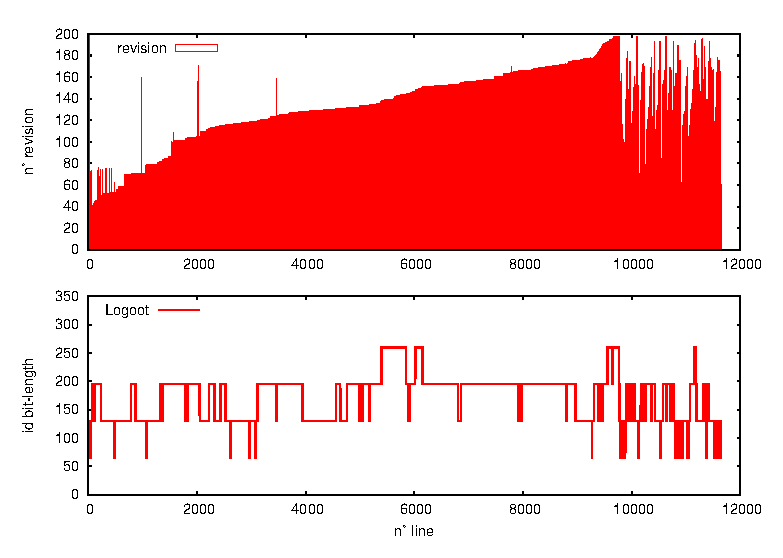
\includegraphics[width=0.48\textwidth]{./img/lseq/compliant.eps}}
  \hspace{10pt}
  \subfloat[Comportement d'édition inattendu]
  [\label{fig:lseq:motivating}Le comportement d'édition va à l'encontre des attentes
  de la stratégie d'allocation]
  {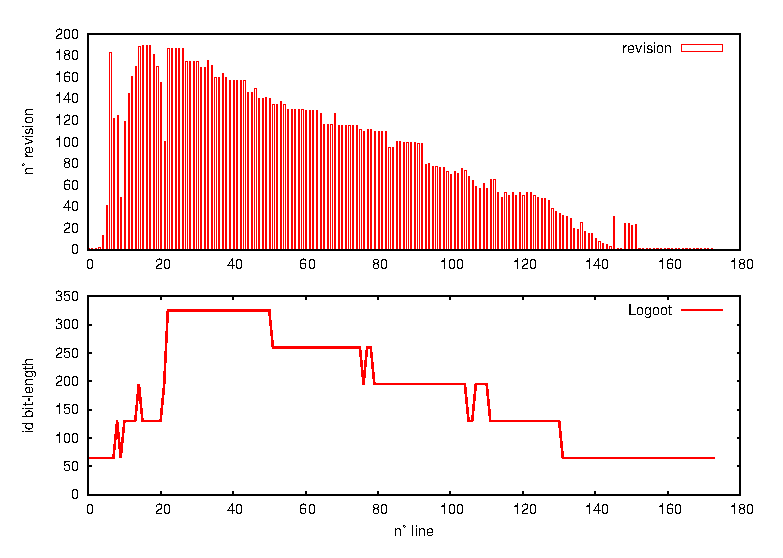
\includegraphics[width=0.48\textwidth]{./img/lseq/motivating.eps}}
  \caption{\label{fig:lseq:allocation}Spectre de documents Wikipedia sous différent
    comportements d'édition antagonistes. La figure du haut représente la
    révision à laquelle la ligne a été insérée, i.e., sa date de naissance.  La
    figure du bas représente la taille de l'identifiant associé à chaque ligne.}
\end{figure*}

Les figures~\ref{fig:lseq:compliant} et~\ref{fig:lseq:motivating} montrent deux
comportements d'éditions présent sur des pages extraites de Wikipedia. La partie
supérieure de ces figures donne une vue globale du comportement d'édition sur la
page. Elle indique la numéro de la révision à laquelle une ligne a été
insérée. Ainsi, plus une barre est haute, plus la ligne a été insérée
récemment. Le spectre de la figure~\ref{fig:lseq:compliant} montre que les
nouveaux éléments de la séquence sont principalement ajoutés en fin. À l'opposé,
le spectre de la figure~\ref{fig:lseq:motivating} montre que les nouveaux
éléments de la séquence sont principalement ajoutés en tête. La partie
inférieure de ces figures montre la taille de la représentation binaire de
l'identifiant associé à chaque élément du document. \TODO{Présenter la stratégie
  d'allocation}. Ainsi, nous observons que les identifiants dans le document
comportant 12k lignes mais principalement édité en fin a des identifiants
n'excédant pas 256 bits. En revanche, le document possédant seulement 170 lignes
édité en tête a des identifiants atteignant déjà les 320 bits.

\TODO{Définition du problème}

%%% Local Variables:
%%% mode: latex
%%% TeX-master: "../../paper"
%%% End:

%%
\section{LSEQ : une stratégie d'allocation polylogarithmique}

\LSEQ (abréviation pour \emph{polyLogarithimic SEQuence}) est une stratégie
d'allocation d'identifiants dont la taille est variable à la génération. Pour
générer ses identifiants immuables et uniques, \LSEQ utilise un arbre
exponentiel comme structure de données, deux sous-stratégies d'allocations avec
objectifs antagonistes, et un composant permettant de choisir la stratégie.

\subsection{Principe général}

Le principe général de \LSEQ consiste à amortir les mauvais choix d'identifiants
par un ensemble suffisant d'identifiants dont la taille est
satisfaisante. Puisqu'il n'existe pas de stratégie d'allocation parfaite sans
connaissance préalable de la séquence d'édition, \LSEQ cherche a être assez
général pour gérer la plupart des comportements d'édition.


\subsection{Arbre exponentiel}

Un arbre exponentiel est une structure d'arbre dont chaque élément de l'arbre
possède k-fois plus de fils que son parent. Par exemple, si l'on fixe $k$ à $2$,
un élément dont le parent possède $4$ fils en possède $8$. Dans ce cas, il y a
une augmentation quadratique du nombre de fils en fonction de la profondeur qui
s'ajoute à l'augmentation commune de l'arbre.

\TODO{figure}

Un identifiant \LSEQ est un suite d'entiers représentant le chemin de l'élément
dans l'arbre. Pour encoder cette suite d'entiers


\subsection{Sous-stratégies d'allocation}

\subsection{Choix de stratégie}

%%% Local Variables:
%%% mode: latex
%%% TeX-master: "../../paper"
%%% End:

%%
\section{Experimentations}

\subsection{Simulations}

%%% Local Variables:
%%% mode: latex
%%% TeX-master: "../../paper"
%%% End:

%%
\section{Conclusion}
\label{lseq:sec:conclusion}

%%% Local Variables:
%%% mode: latex
%%% TeX-master: "../../paper"
%%% End:


%%% Local Variables:
%%% mode: latex
%%% TeX-master: "../../paper"
%%% End:
